% \documentclass{article}
% 
% 
% % \usepackage{arxiv} # uncomment for preprint
% 
% \usepackage[utf8]{inputenc} % allow utf-8 input
% \usepackage[T1]{fontenc}    % use 8-bit T1 fonts
% % \usepackage{hyperref}       % hyperlinks
% \usepackage{url}            % simple URL typesetting
% \usepackage{booktabs}       % professional-quality tables
% \usepackage{amsfonts}       % blackboard math symbols
% \usepackage{nicefrac}       % compact symbols for 1/2, etc.
% \usepackage{microtype}      % microtypography
% \usepackage{lipsum}
% \usepackage{graphicx}
% \let\subcaption\relax
% \usepackage{caption}
% \usepackage{subcaption}
% % \usepackage{subfigure}
% \usepackage{amsmath}
% % \usepackage{amssymb}
% \usepackage{amsthm}
% \usepackage{algorithmic}
% \usepackage{hyperref}
% \usepackage{xr}
% % \usepackage{subfig}
% \usepackage{xcolor}
% \usepackage{multirow}
% 
% \usepackage{placeins}
% % \usepackage{algpseudocode}
% \usepackage{algorithm}
% 
% % \algnewcommand\algorithmicforeach{\textbf{foreach}}
% % \algdef{S}[FOR]{ForEach}[1]{\algorithmicforeach\ #1\ \algorithmicdo}
% 
% 
% \usepackage{hyperref}
% 
% 
% \begin{document}

% \renewcommand{\thetable}{S\arabic{table}}
% 
% \renewcommand{\thefigure}{S\arabic{figure}}

\section{Supplementary Results}

\begin{figure}[ht!]
    \centering
    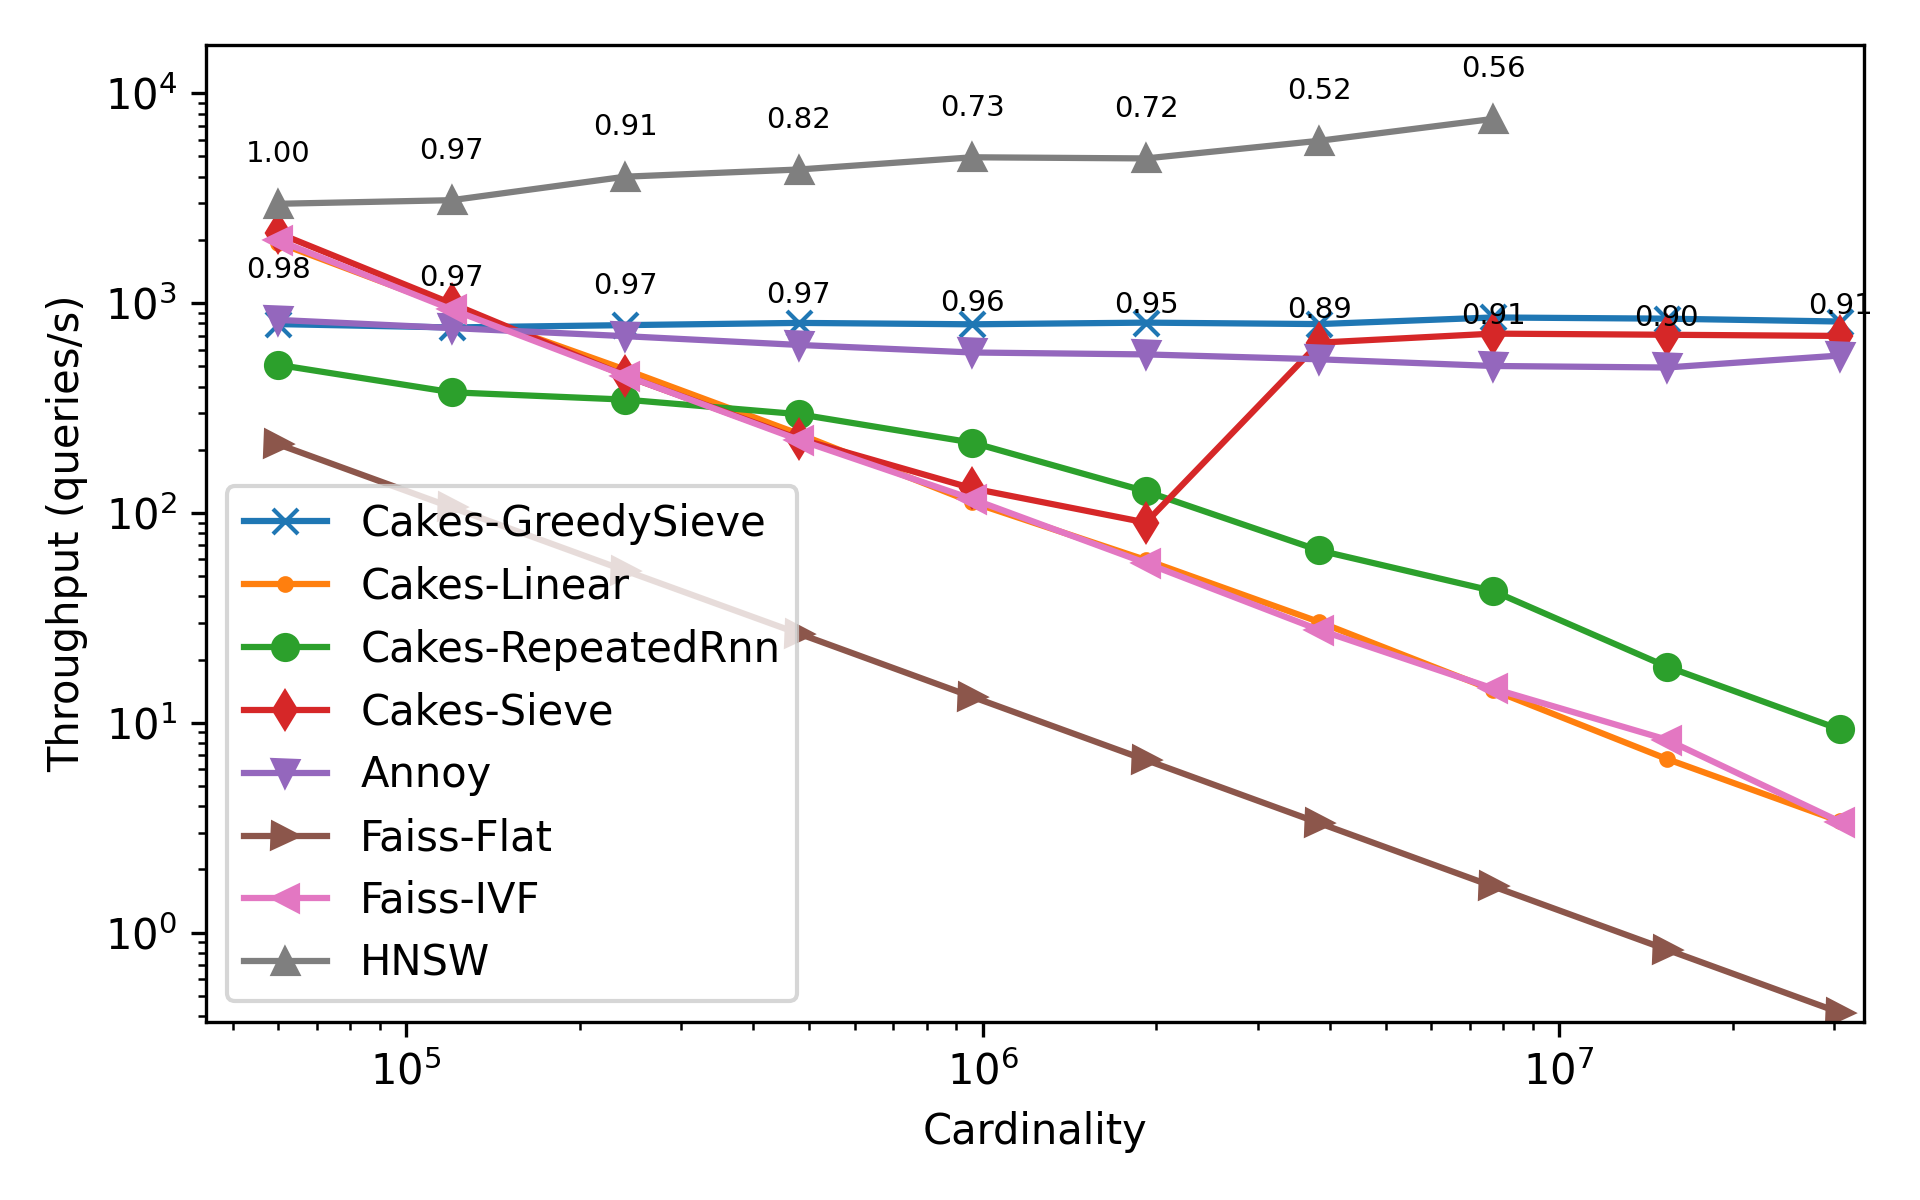
\includegraphics[width=3.4in]{plots/fashion-mnist-knn-100.png}
    \caption{
        Scaling behavior of algorithms on fashion-mnist with $k=100$. 
    }
    \label{fig:supplement:fashion-mnist-k-100}
\end{figure}

\begin{figure}[ht!]
    \centering
    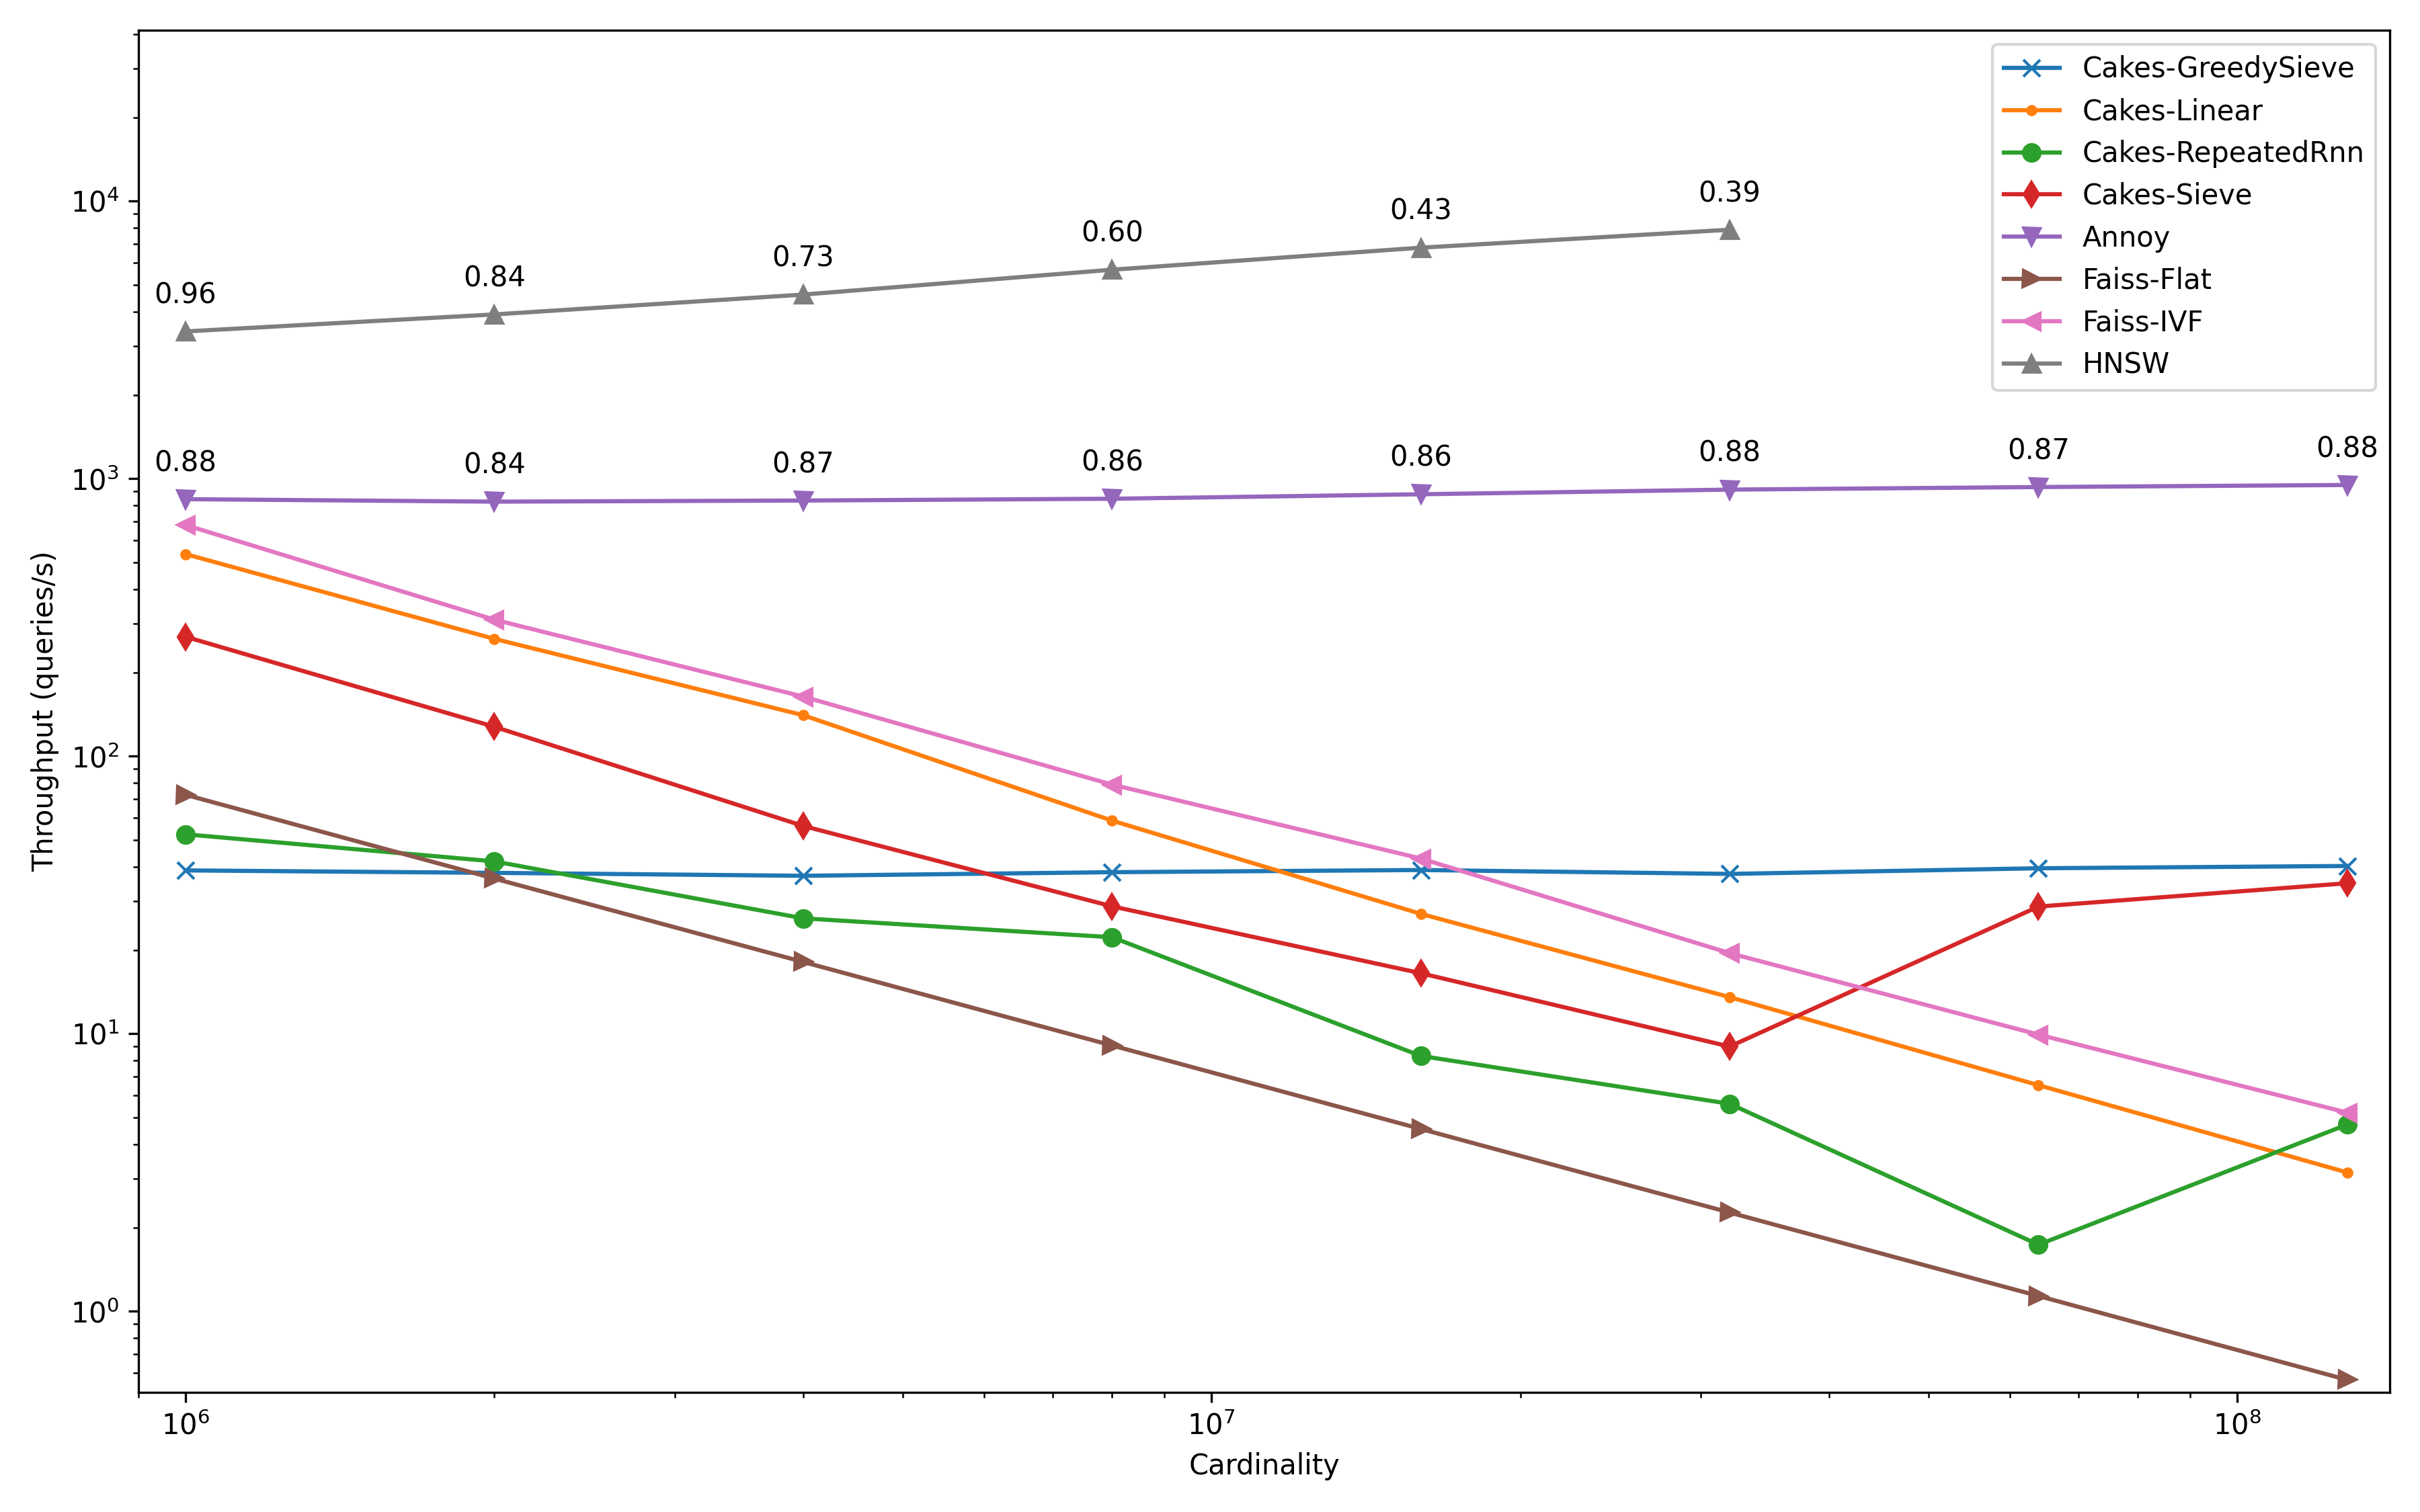
\includegraphics[width=3.4in]{plots/sift-knn-100.png}
    \caption{
        Scaling behavior of algorithms on sift with $k=100$. 
    }
    \label{fig:supplement:sift-k-100}
\end{figure}

\begin{figure}[ht!]
    \centering
    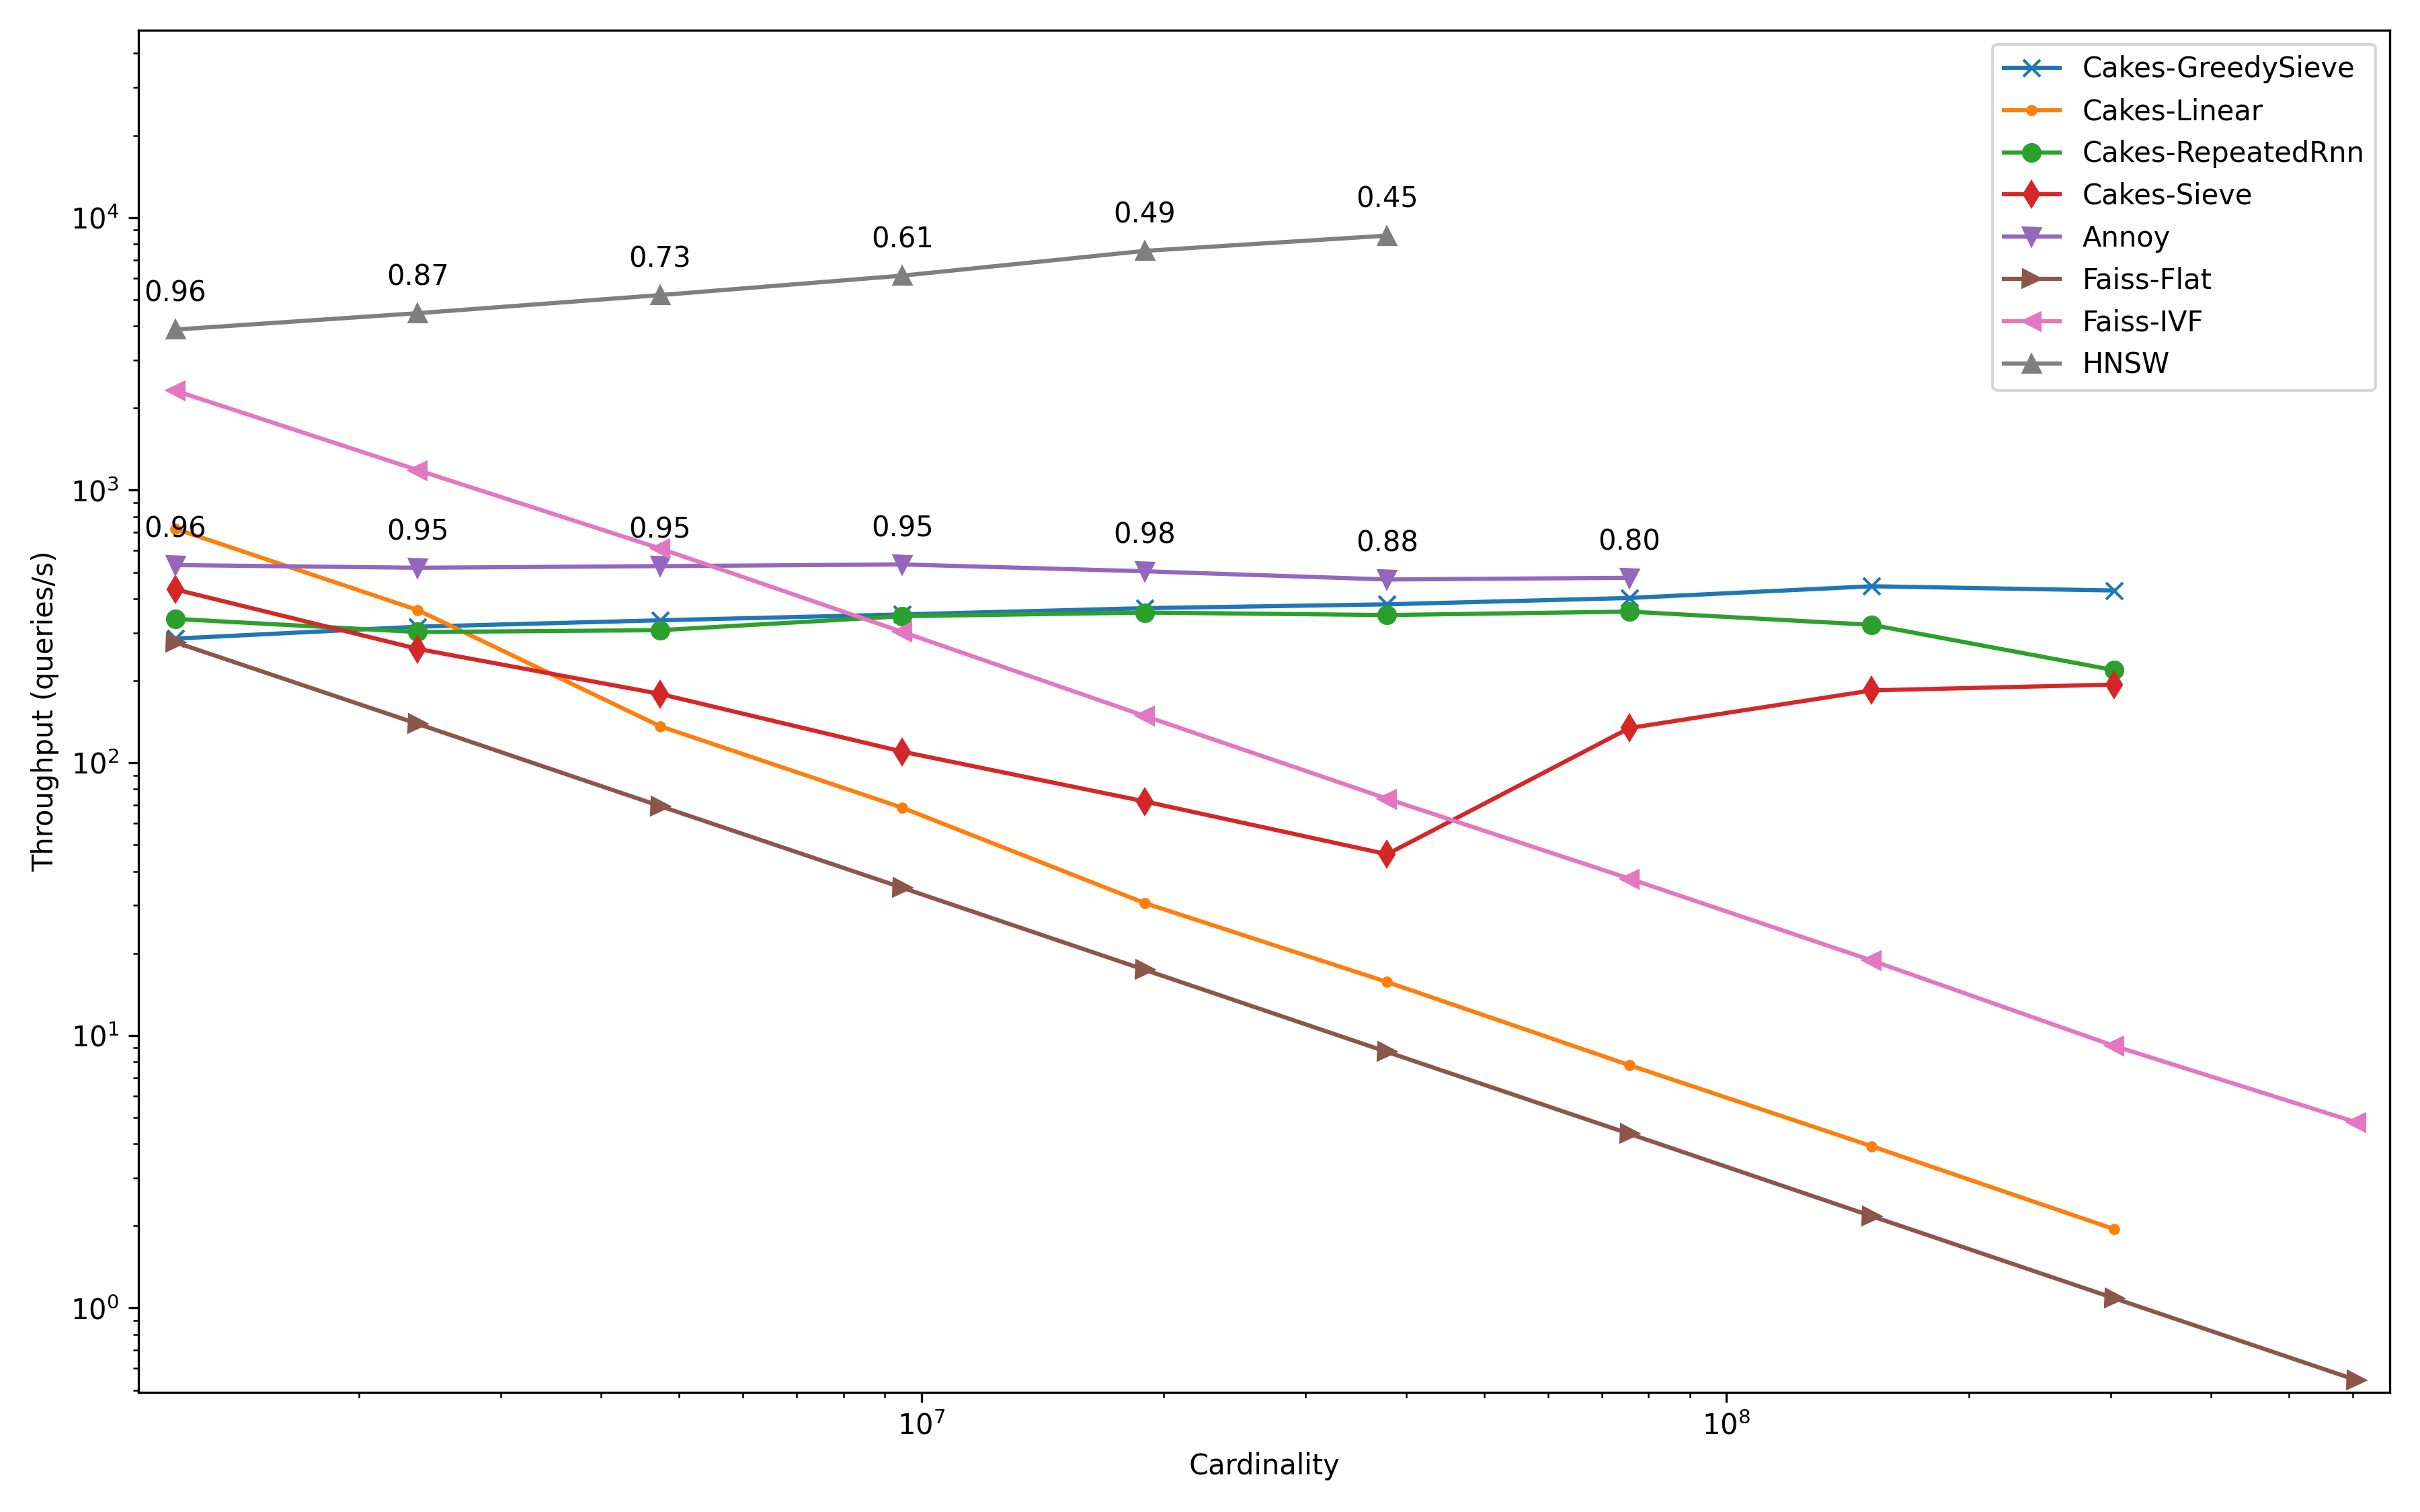
\includegraphics[width=3.4in]{plots/glove-25-knn-100.png}
    \caption{
        Scaling behavior of algorithms on glove-25 with $k=100$. 
    }
    \label{fig:supplement:glove-25-k-100}
\end{figure}

\begin{figure}[ht!]
    \centering
    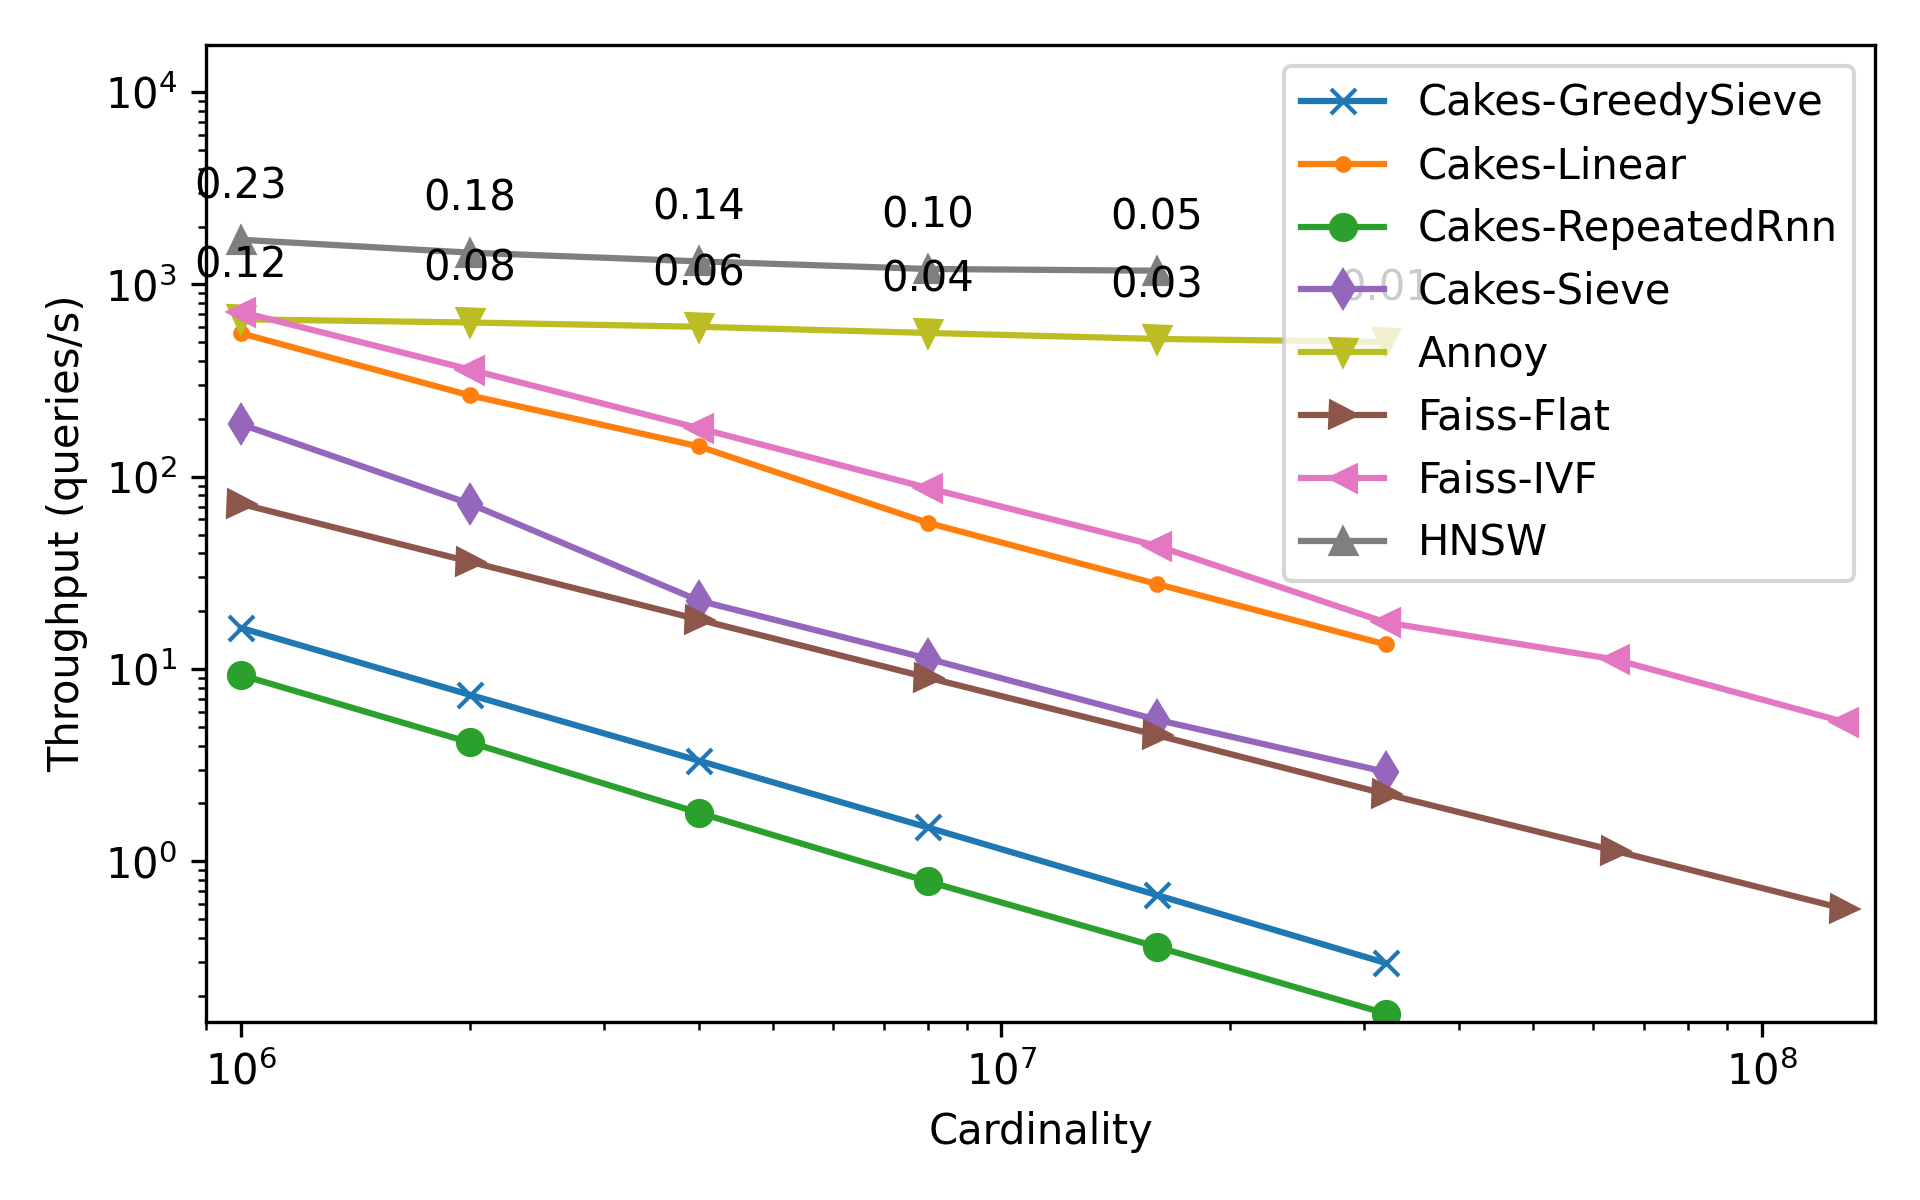
\includegraphics[width=3.4in]{plots/random-knn-100.png}
    \caption{
        Scaling behavior of algorithms on random with $k=100$. 
    }
    \label{fig:supplement:random-k-100}
\end{figure}

\begin{figure}[ht!]
    \begin{subfigure}[b]{0.47\textwidth}
    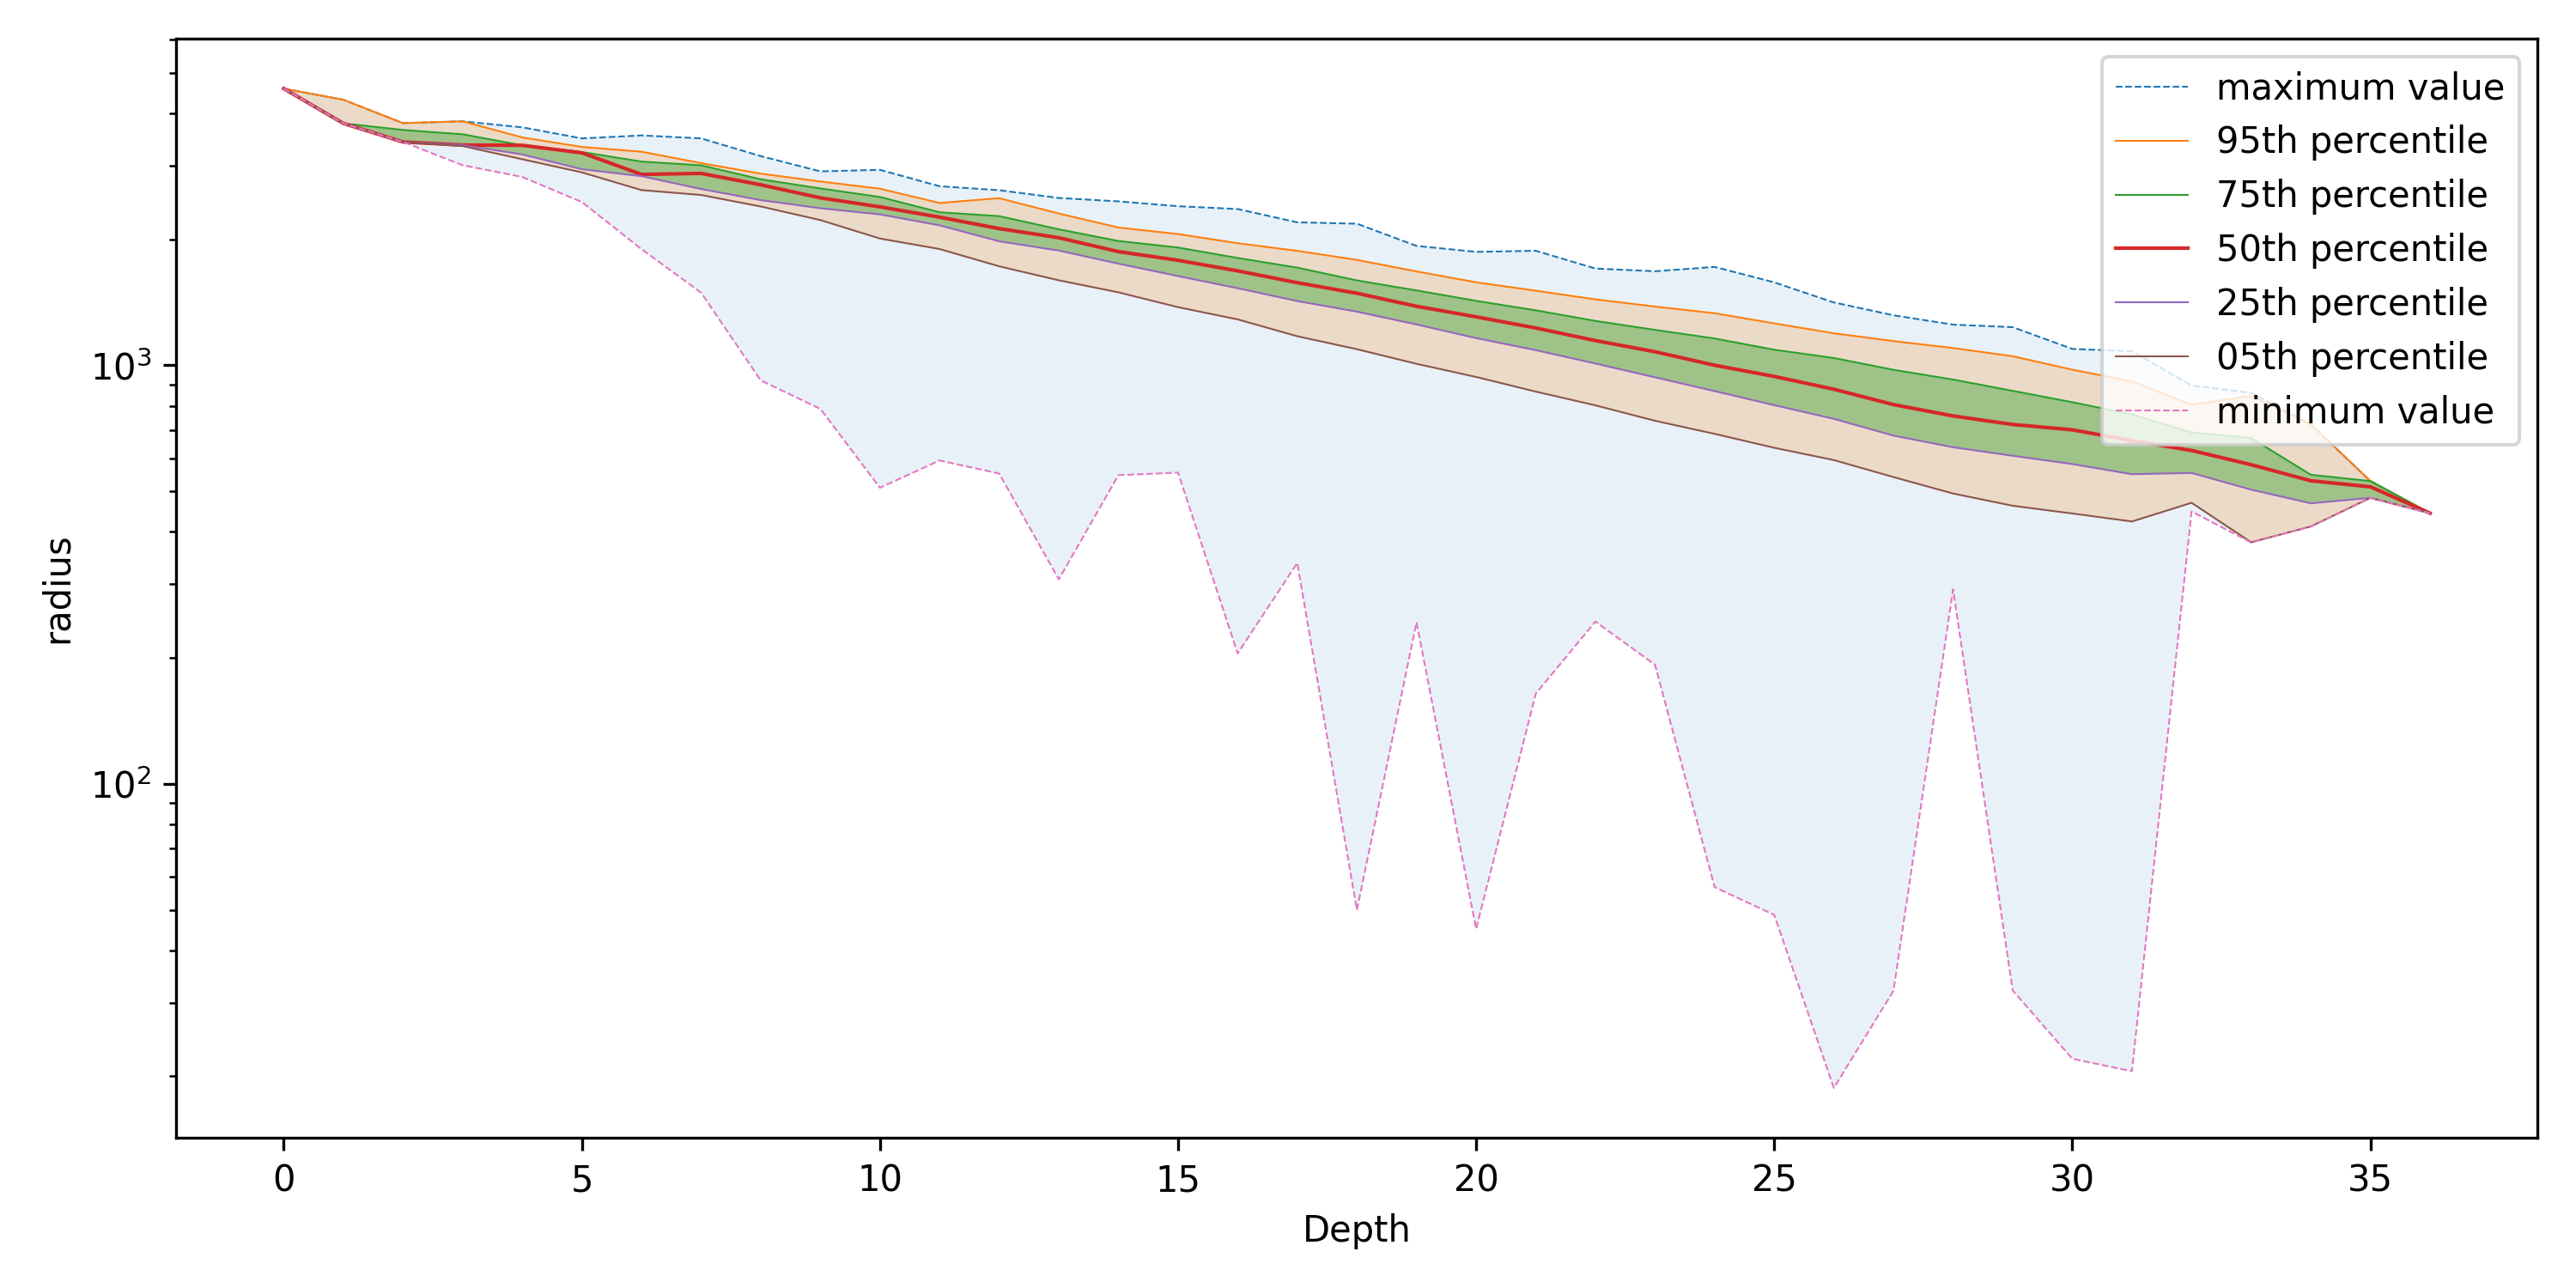
\includegraphics[width=0.95\textwidth]{images/radius/fashion-mnist-60000.png}\\
    \subcaption{Fashion-mnist}
    \label{fig:results:fashion-mnist-radius}
    \end{subfigure}%
    \begin{subfigure}[b]{0.47\textwidth}
    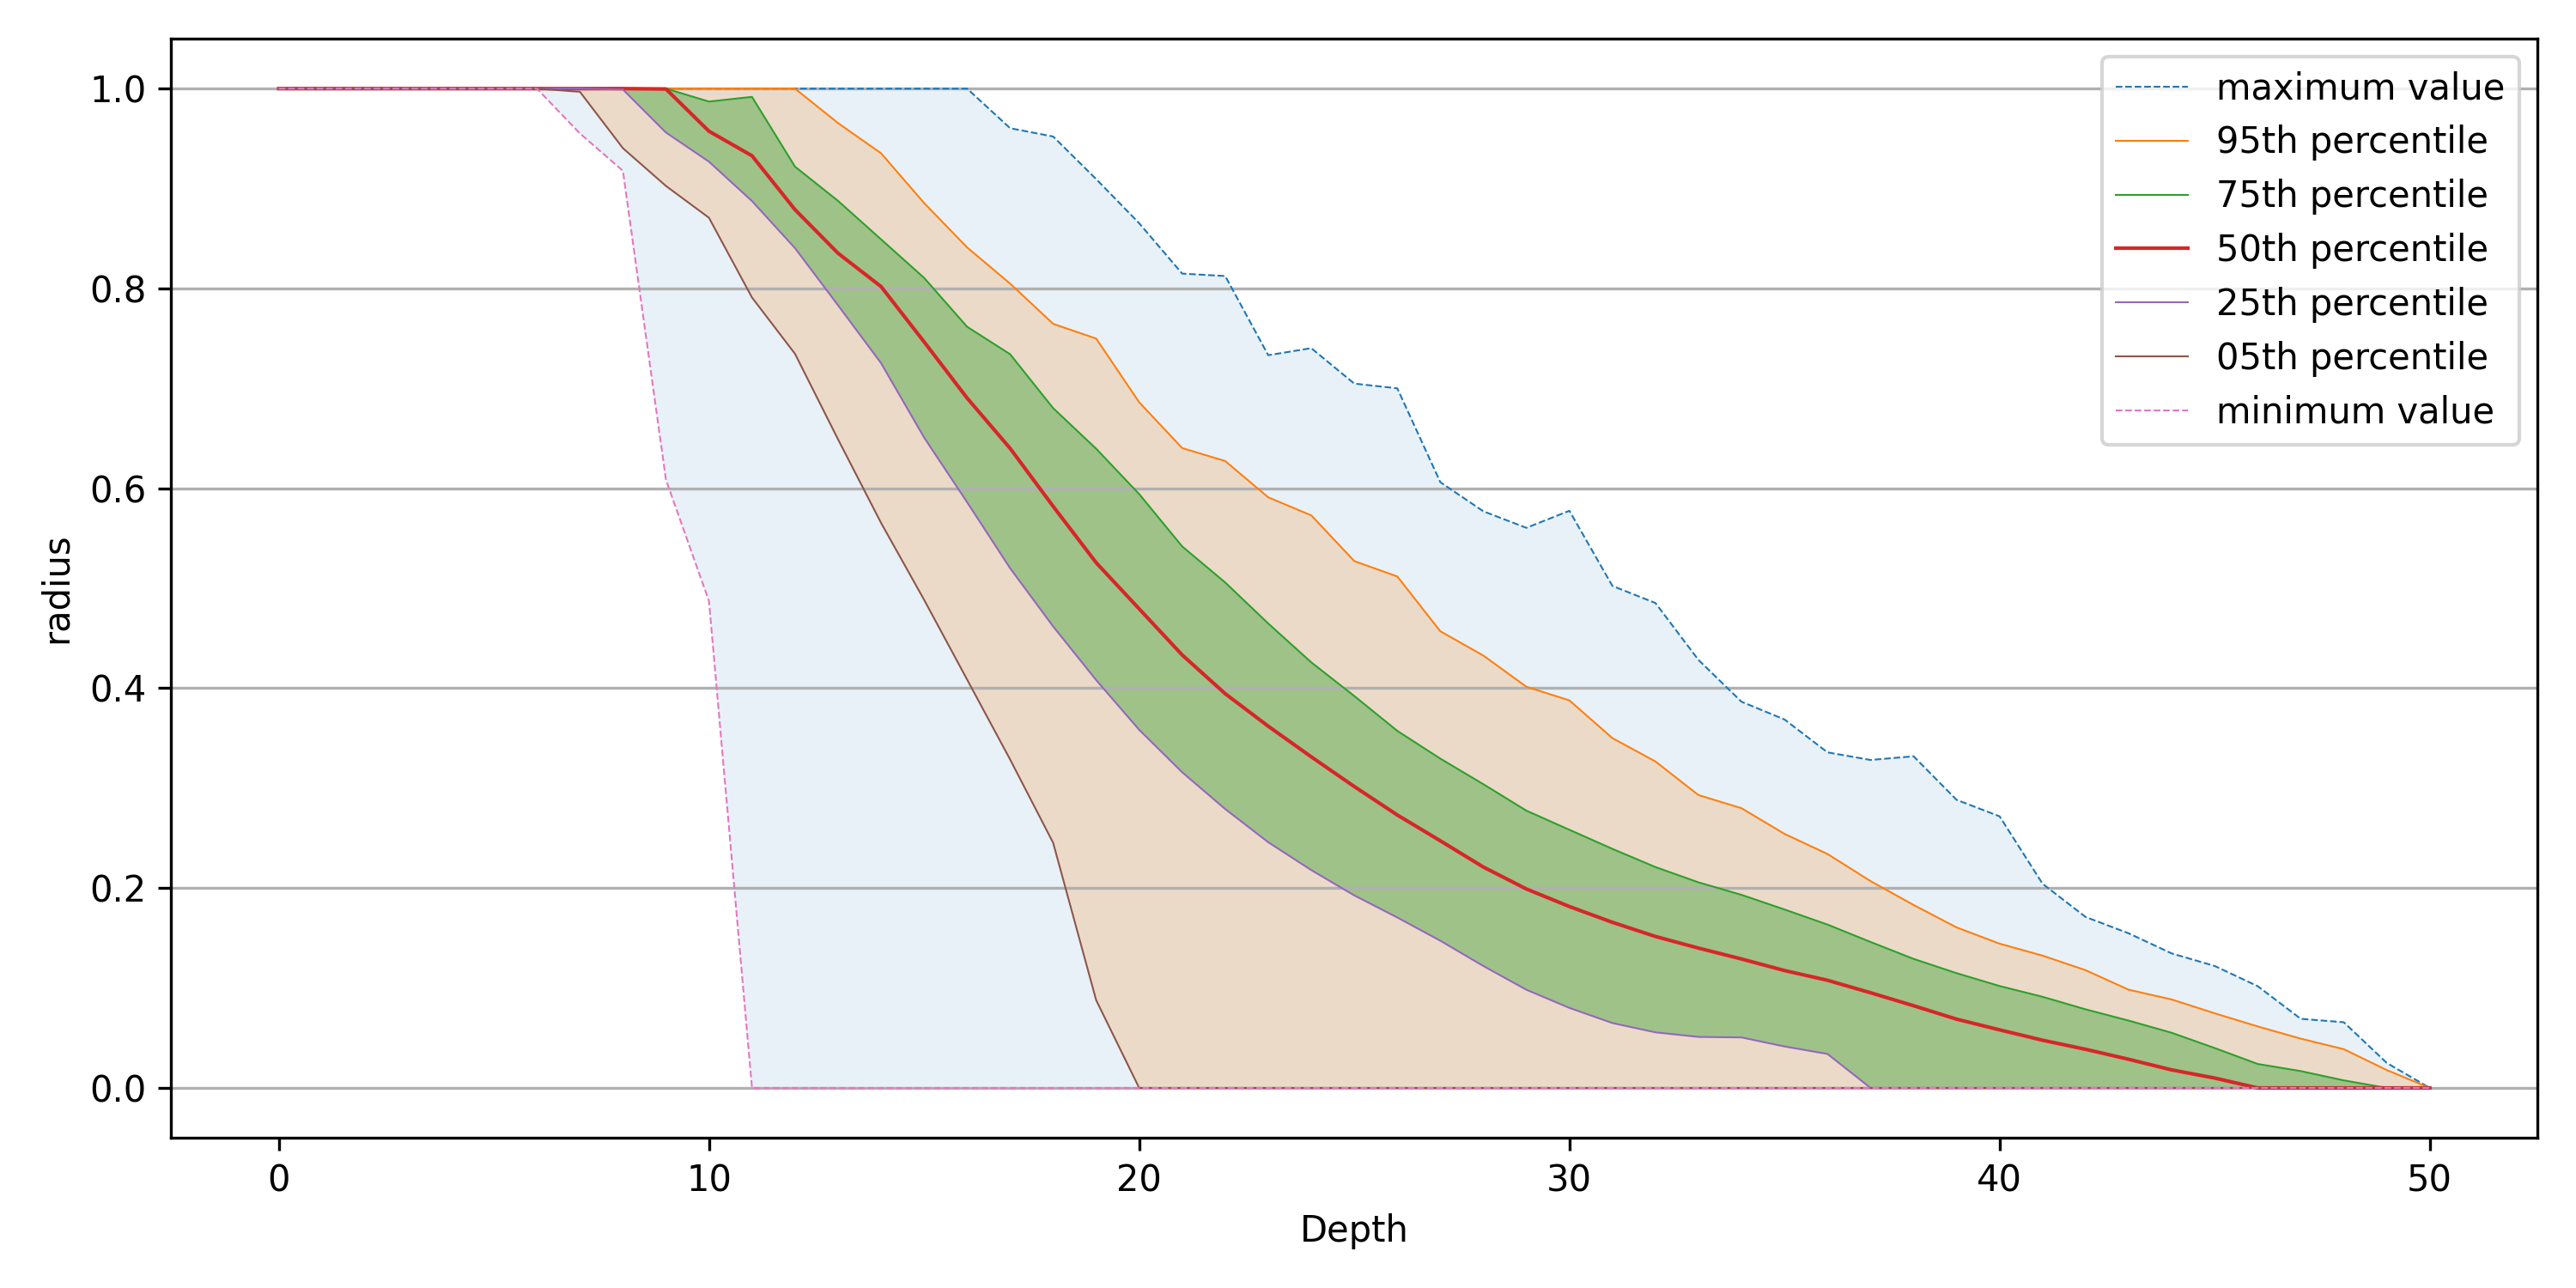
\includegraphics[width=0.95\textwidth]{images/radius/glove-25-1183514.png}\\
    \subcaption{Glove-25}
    \label{fig:results:glove-25-radius}
    \end{subfigure}
    \vspace{1em}
    \\
    \begin{subfigure}[b]{0.47\textwidth}
    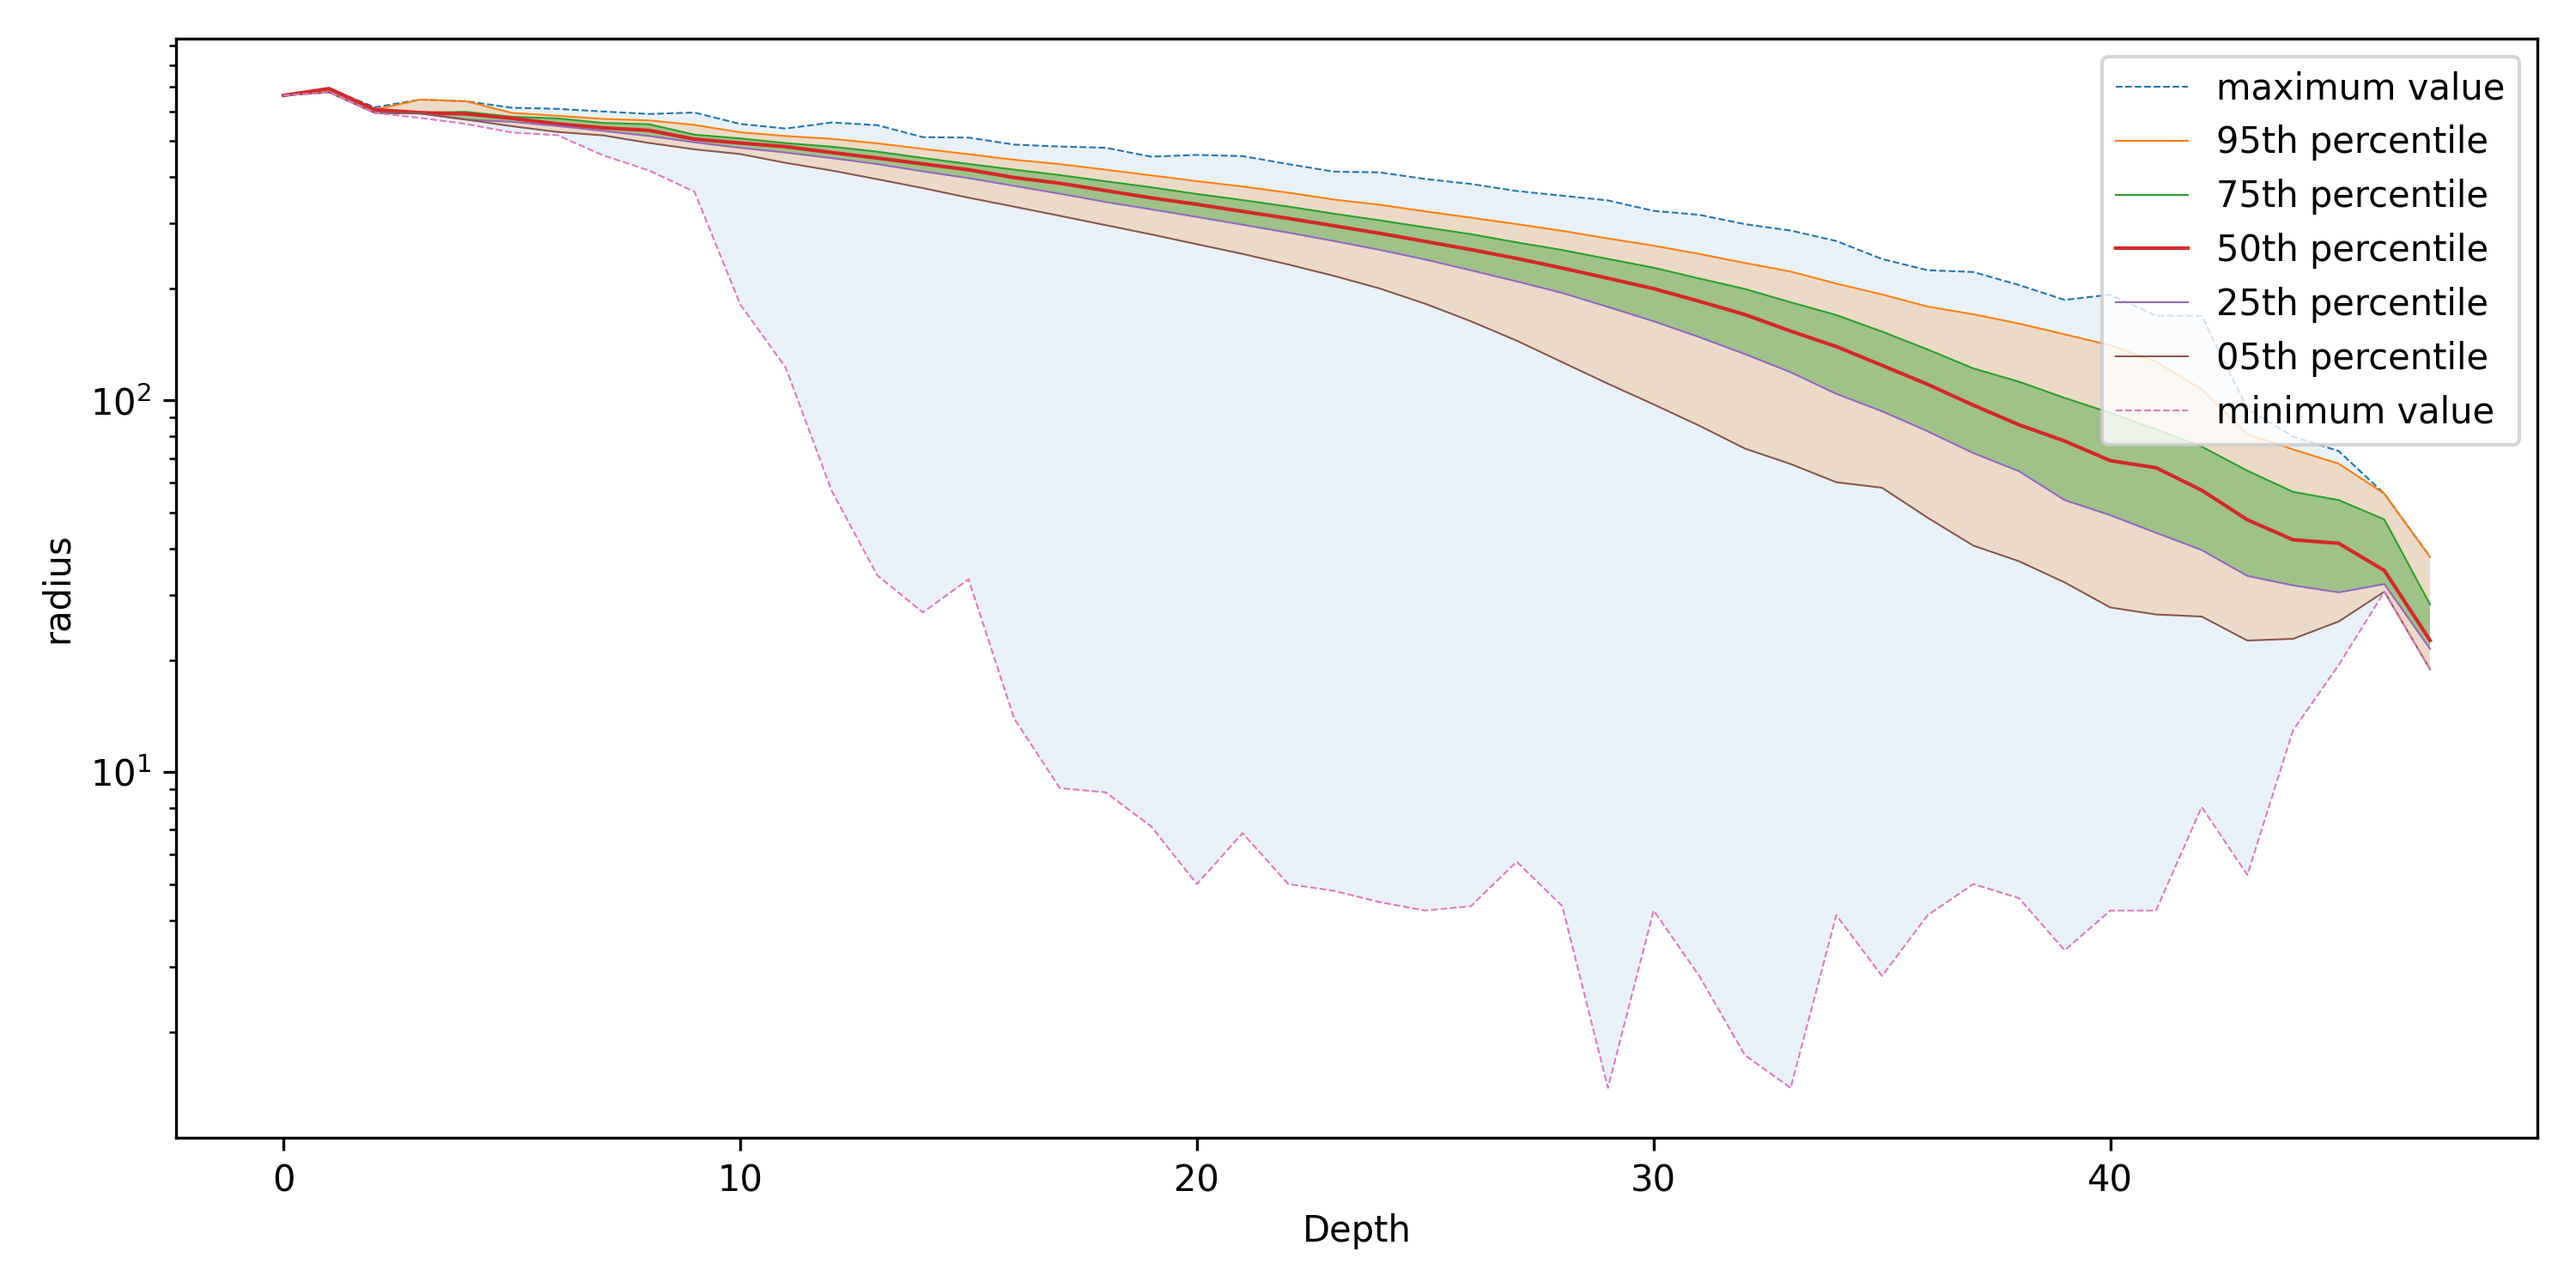
\includegraphics[width=0.95\textwidth]{images/radius/sift-1000000.png}\\
    \subcaption{Sift}
    \label{fig:results:sift-radius}
    \end{subfigure}%
    \begin{subfigure}[b]{0.47\textwidth}
    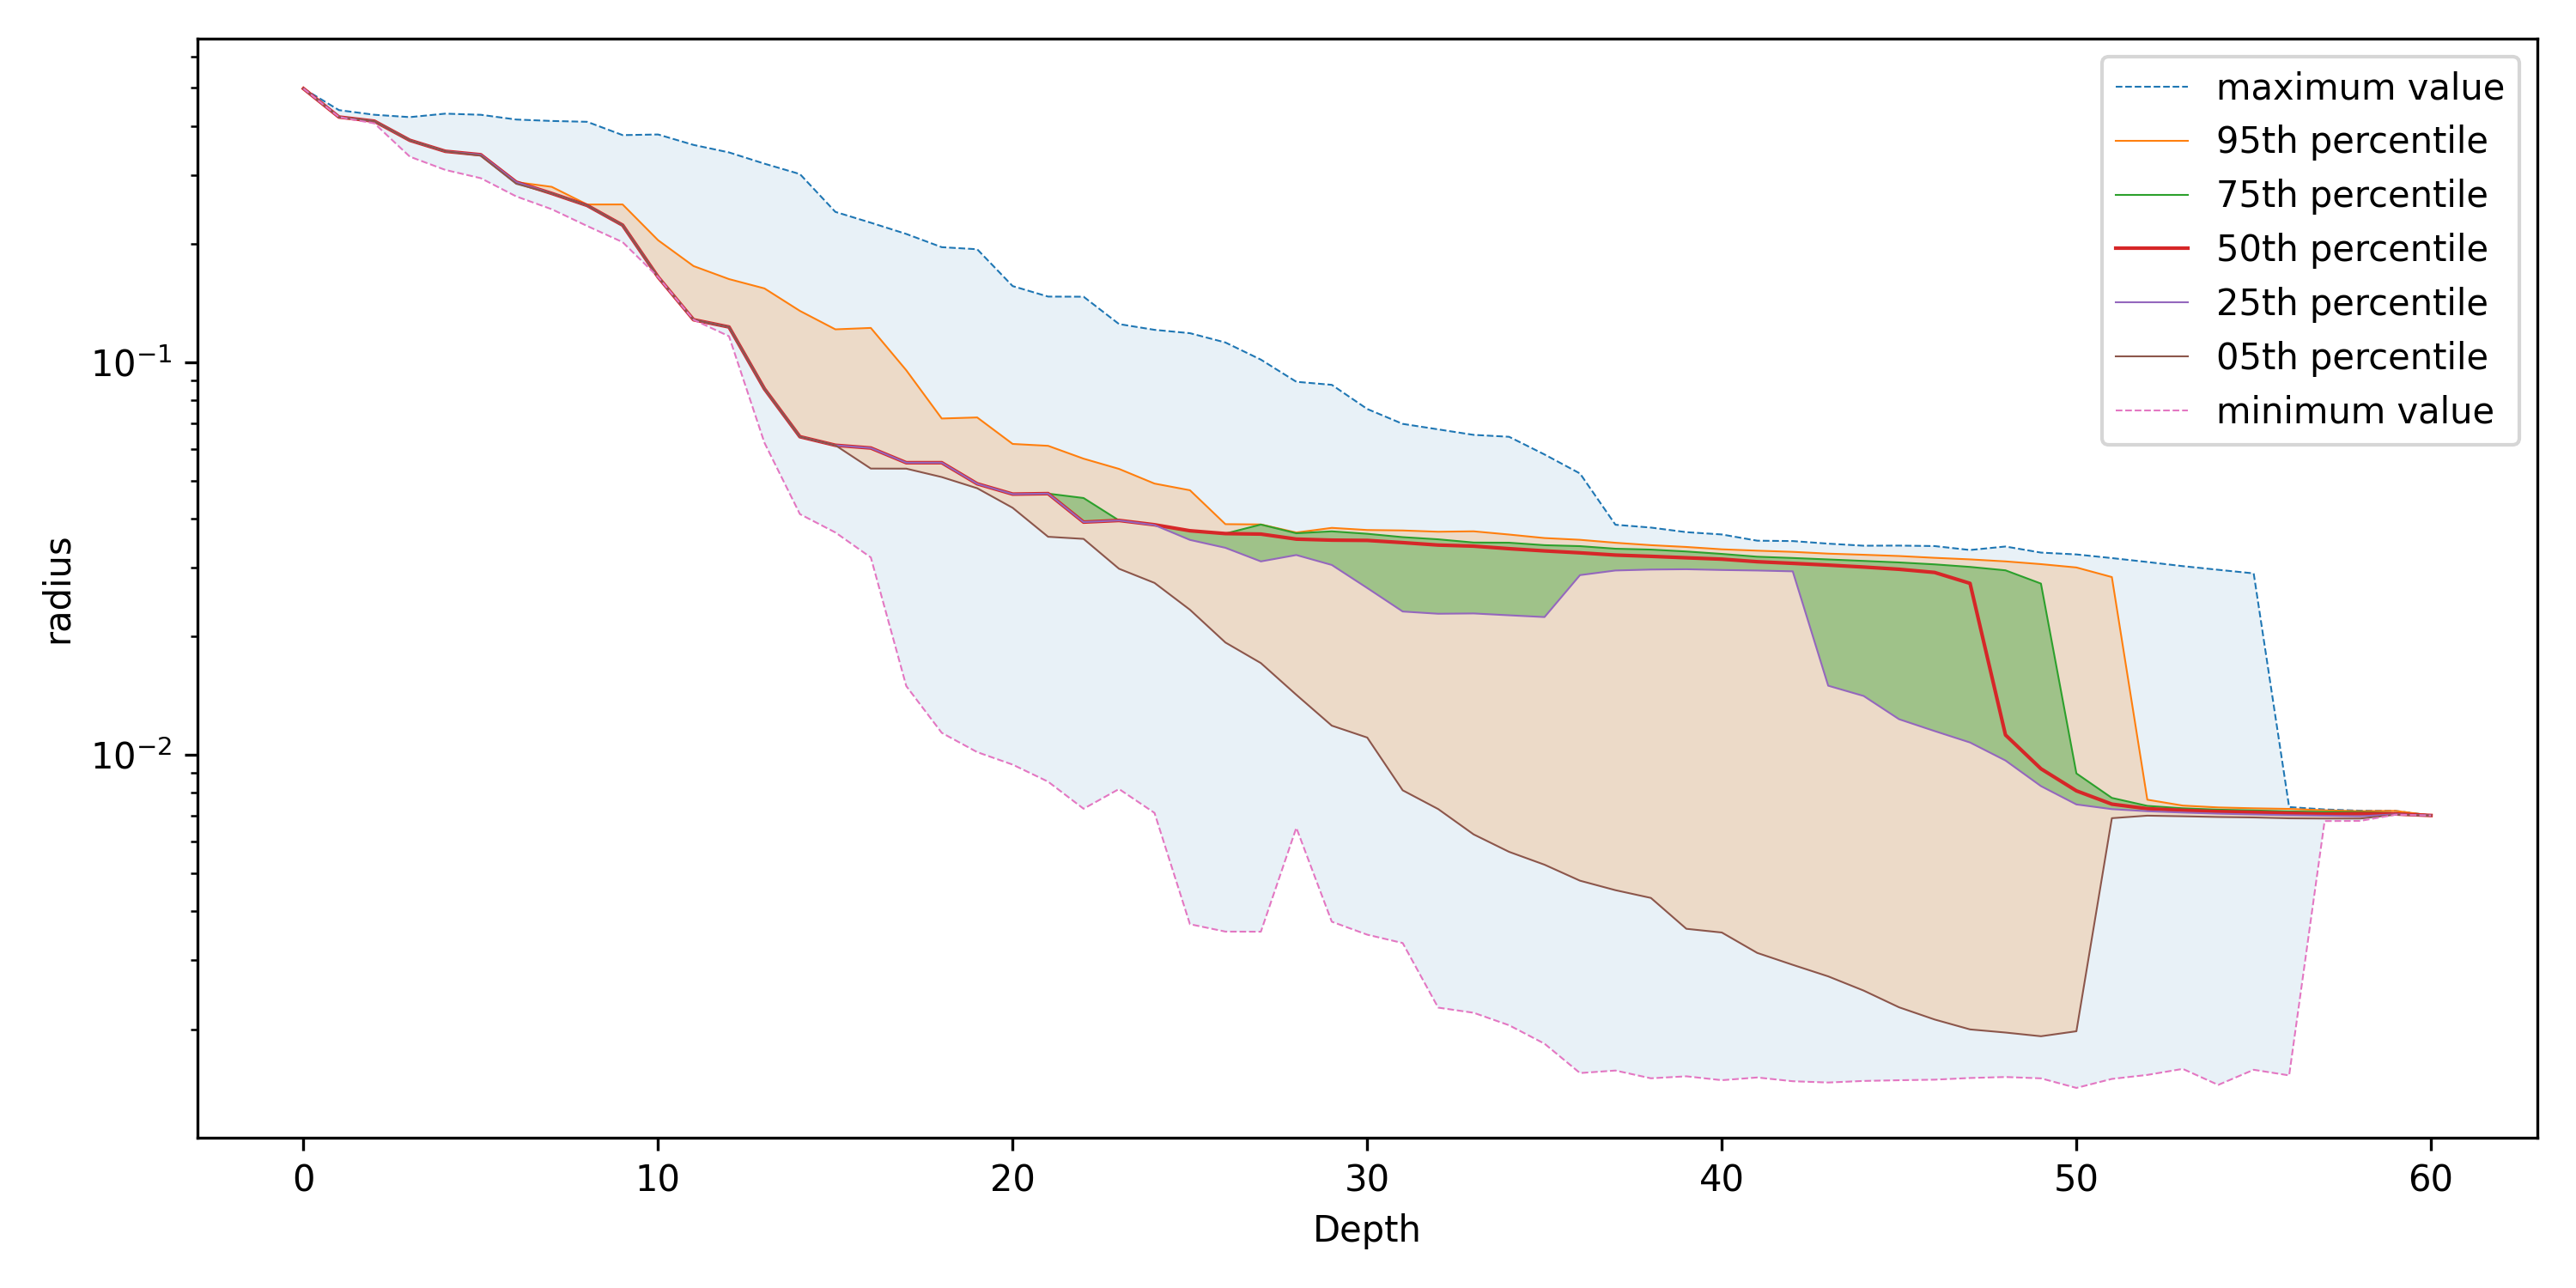
\includegraphics[width=0.95\textwidth]{images/radius/radio-ml-97920.png}\\
    \subcaption{RadioML}
    \label{fig:results:radioml-radius}
    \end{subfigure}%
    \\
    \begin{subfigure}[b]{0.47\textwidth}
    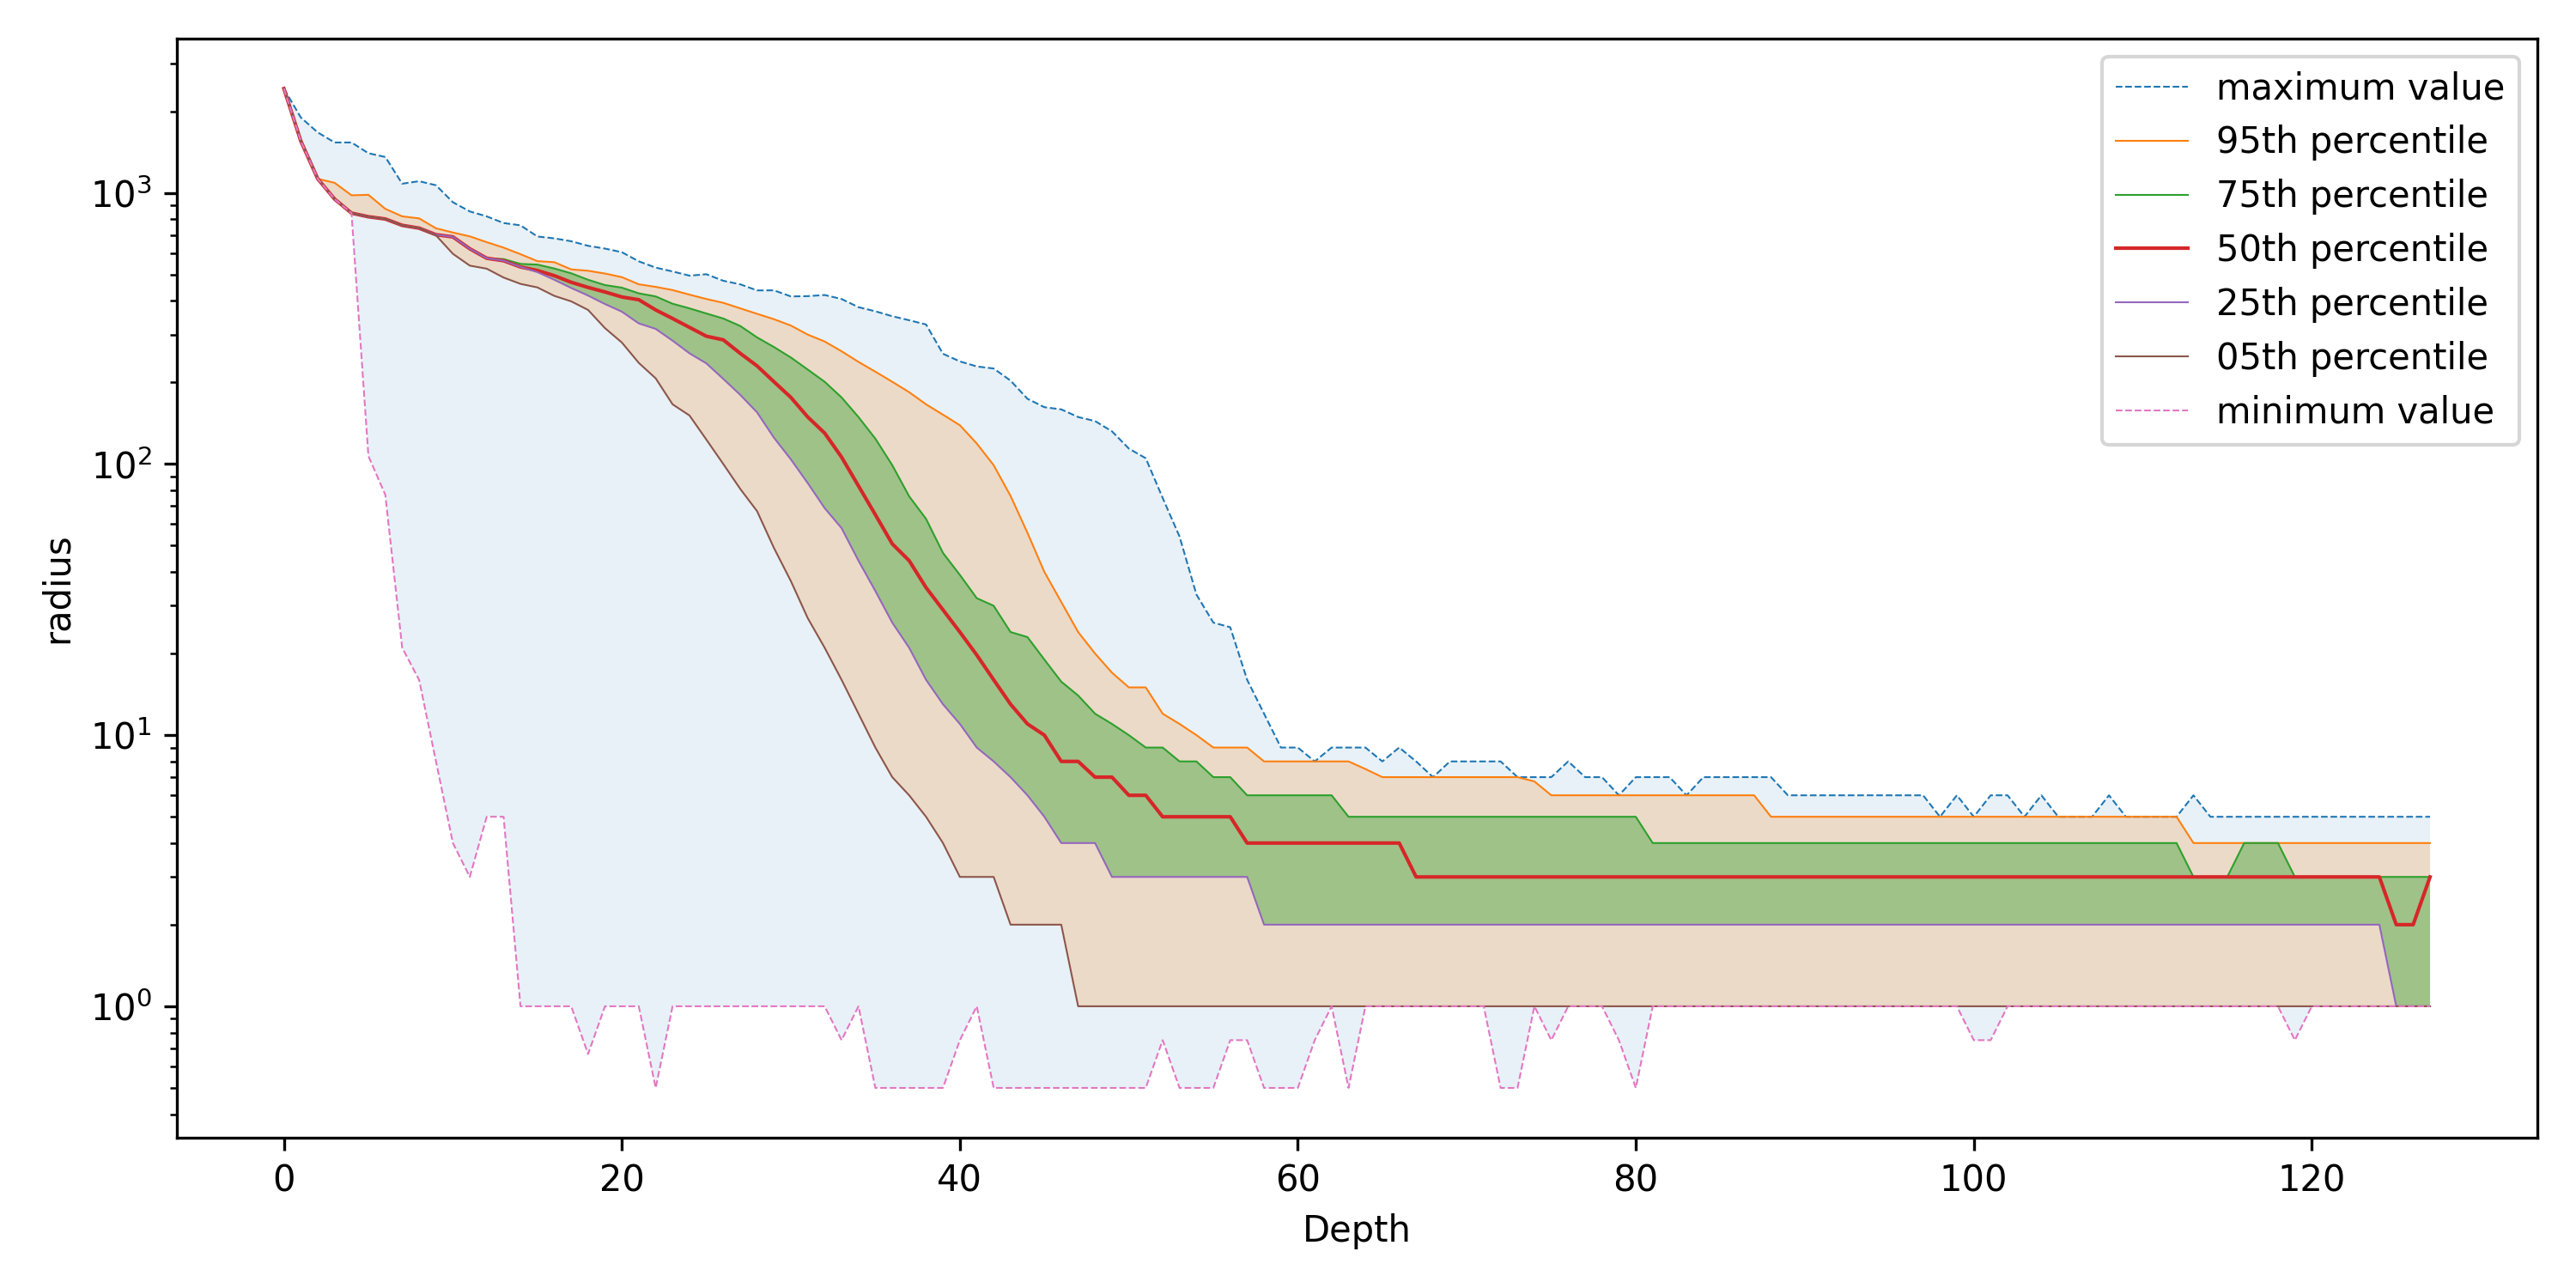
\includegraphics[width=0.95\textwidth]{images/radius/silva-2224640.png}\\
    \subcaption{Silva 18S}
    \label{fig:results:silva-radius}
    \end{subfigure}%  
    \begin{subfigure}[b]{0.47\textwidth}
    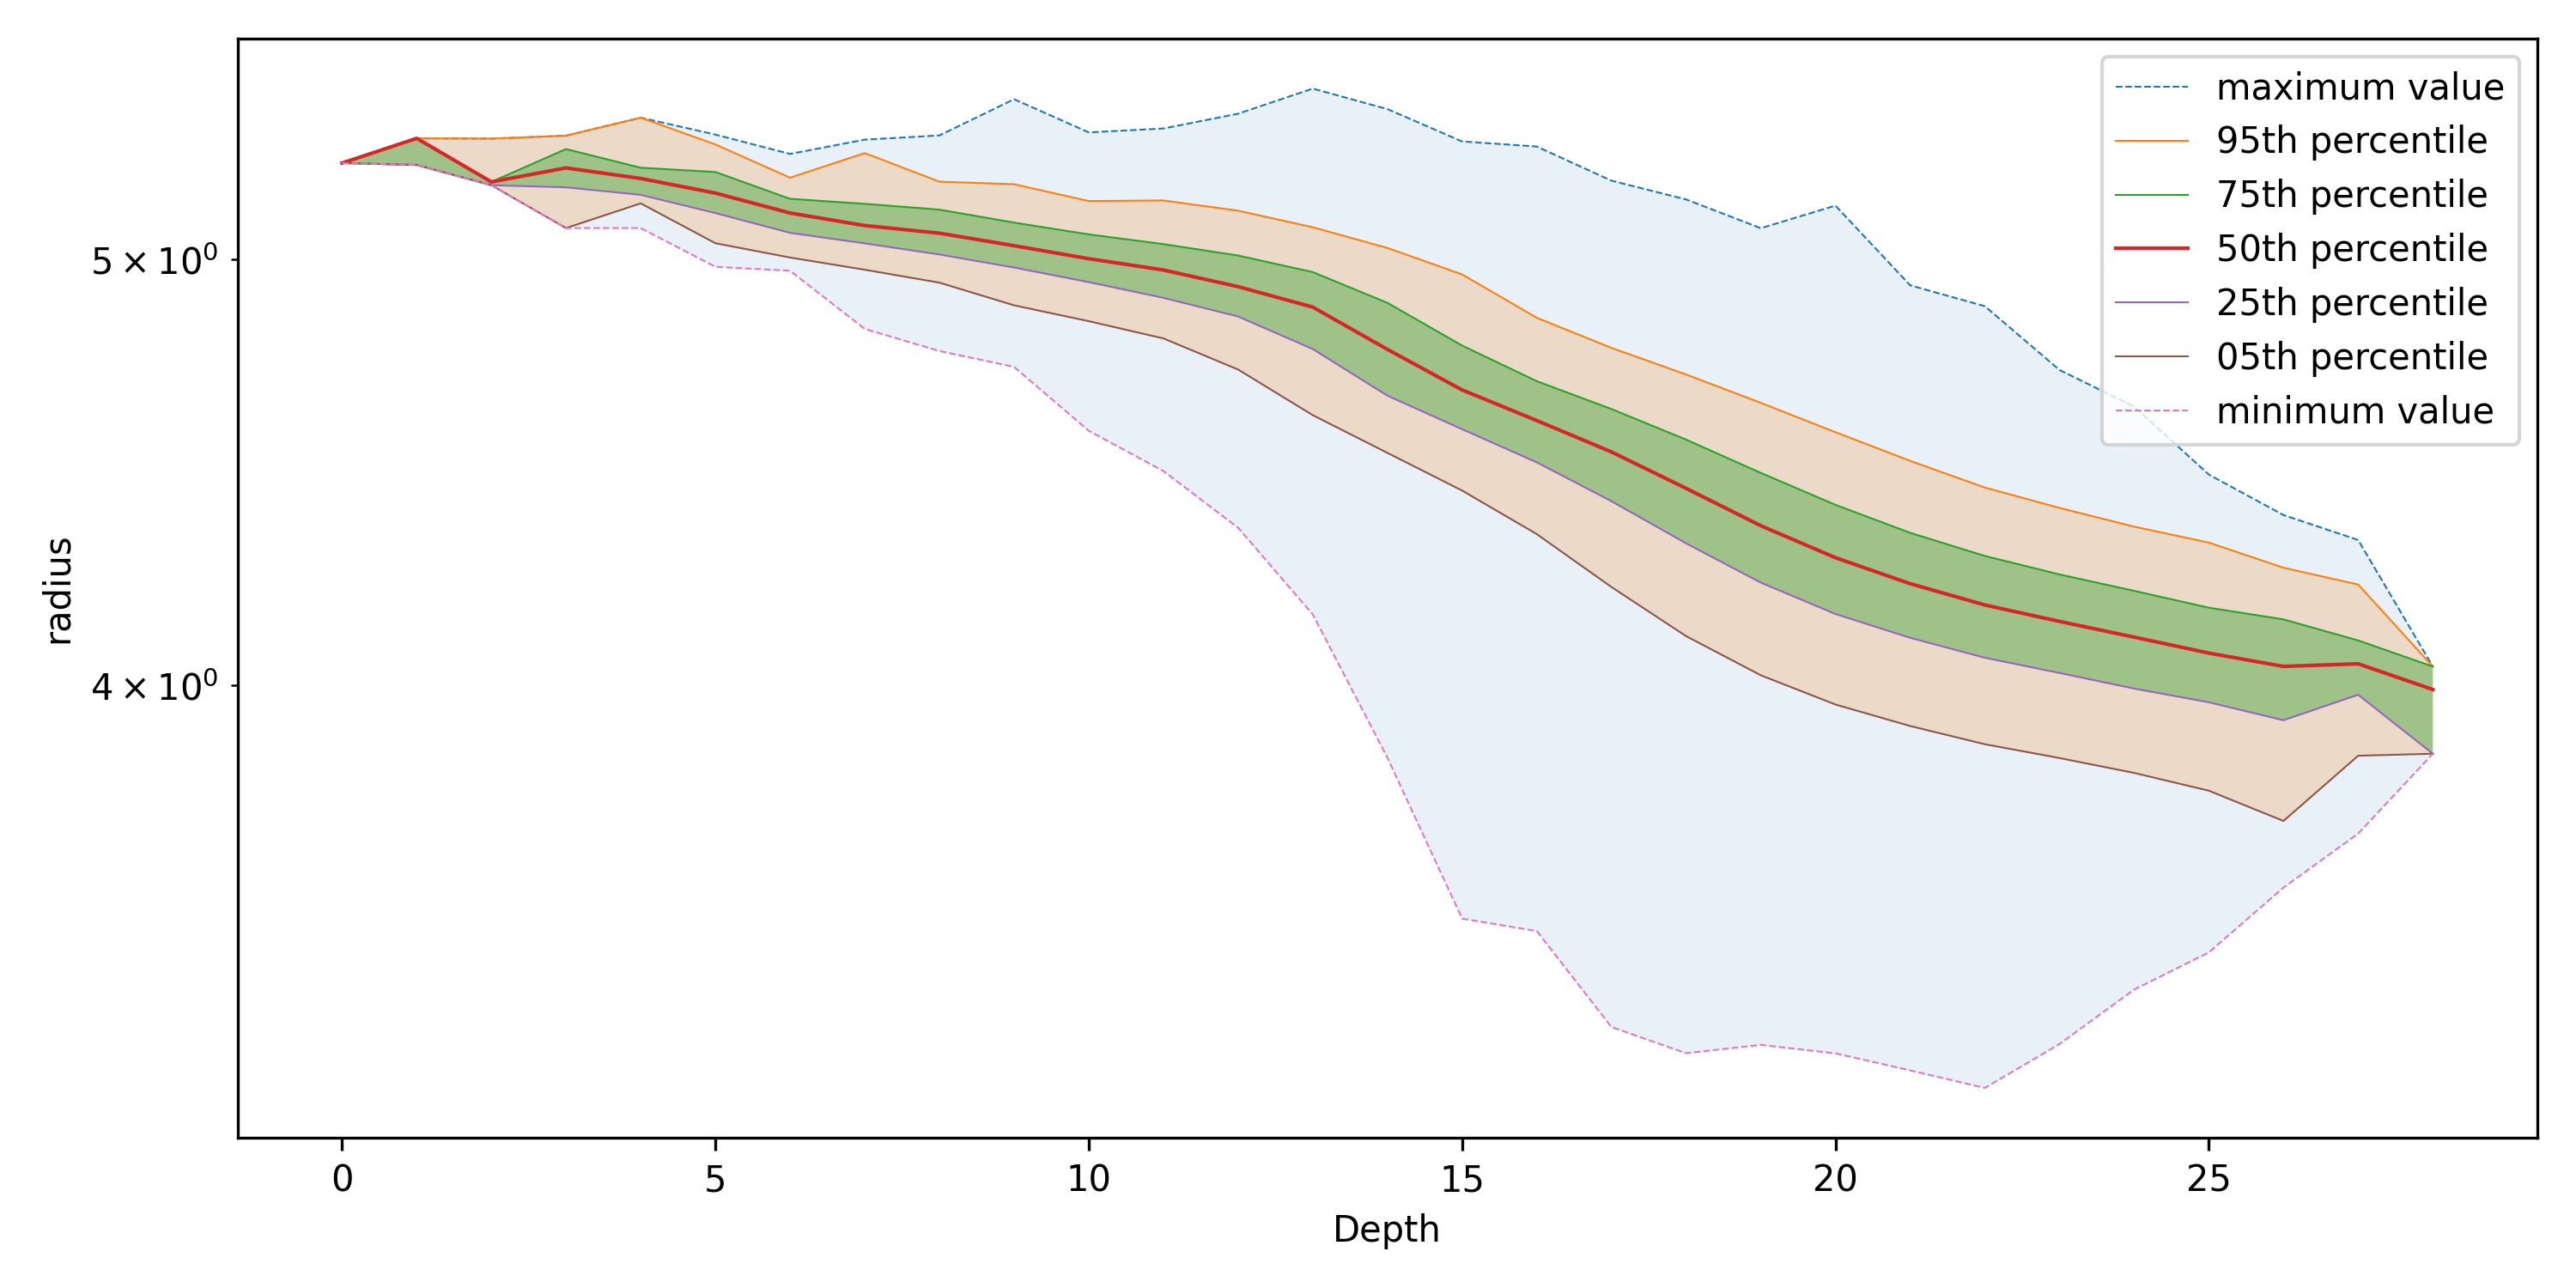
\includegraphics[width=0.95\textwidth]{images/radius/random-1000000.png}\\
    \subcaption{A random dataset}
    \label{fig:results:random-radius}
    \end{subfigure}
    \vspace{1em}
    \caption{Radius vs. cluster depth across six datasets, grouped by decile of radius and weighted by the cardinalities of the clusters.
    The last dataset is randomly generated.}
    \label{fig:results:radius-plots}
\end{figure}

\begin{figure}[ht!]
    \begin{subfigure}[b]{0.47\textwidth}
    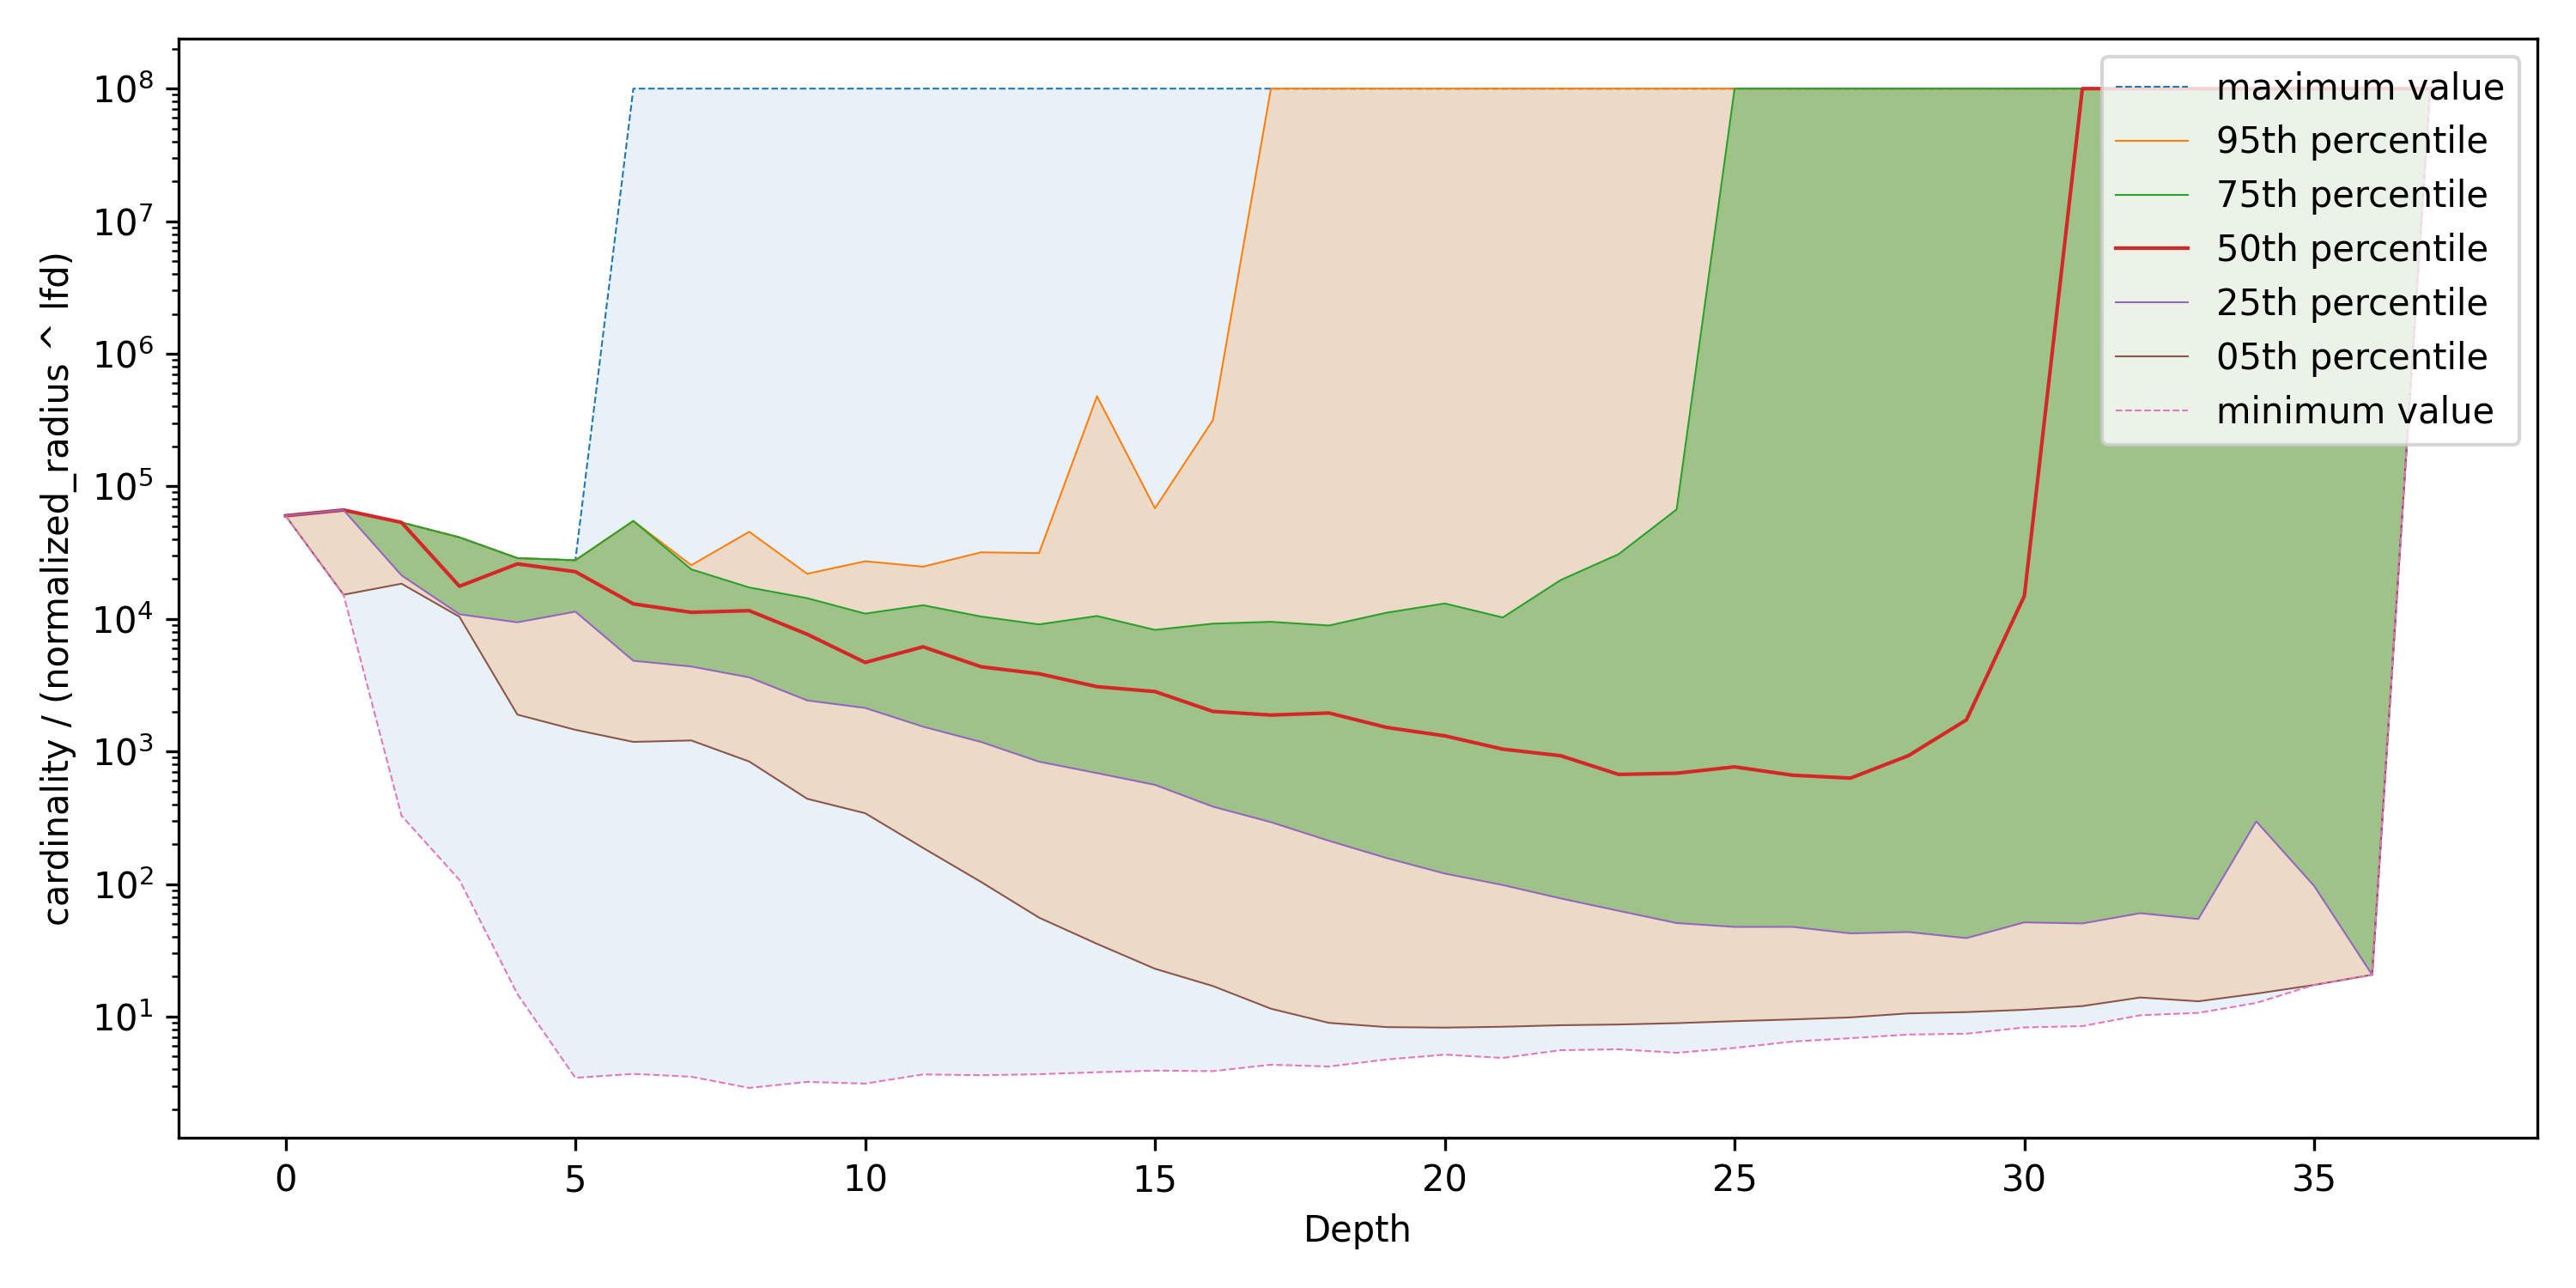
\includegraphics[width=0.95\textwidth]{images/fractal_density/fashion-mnist-60000.png}\\
    \subcaption{Fashion-mnist}
    \label{fig:results:fashion-mnist-fractal_density}
    \end{subfigure}%
    \begin{subfigure}[b]{0.47\textwidth}
    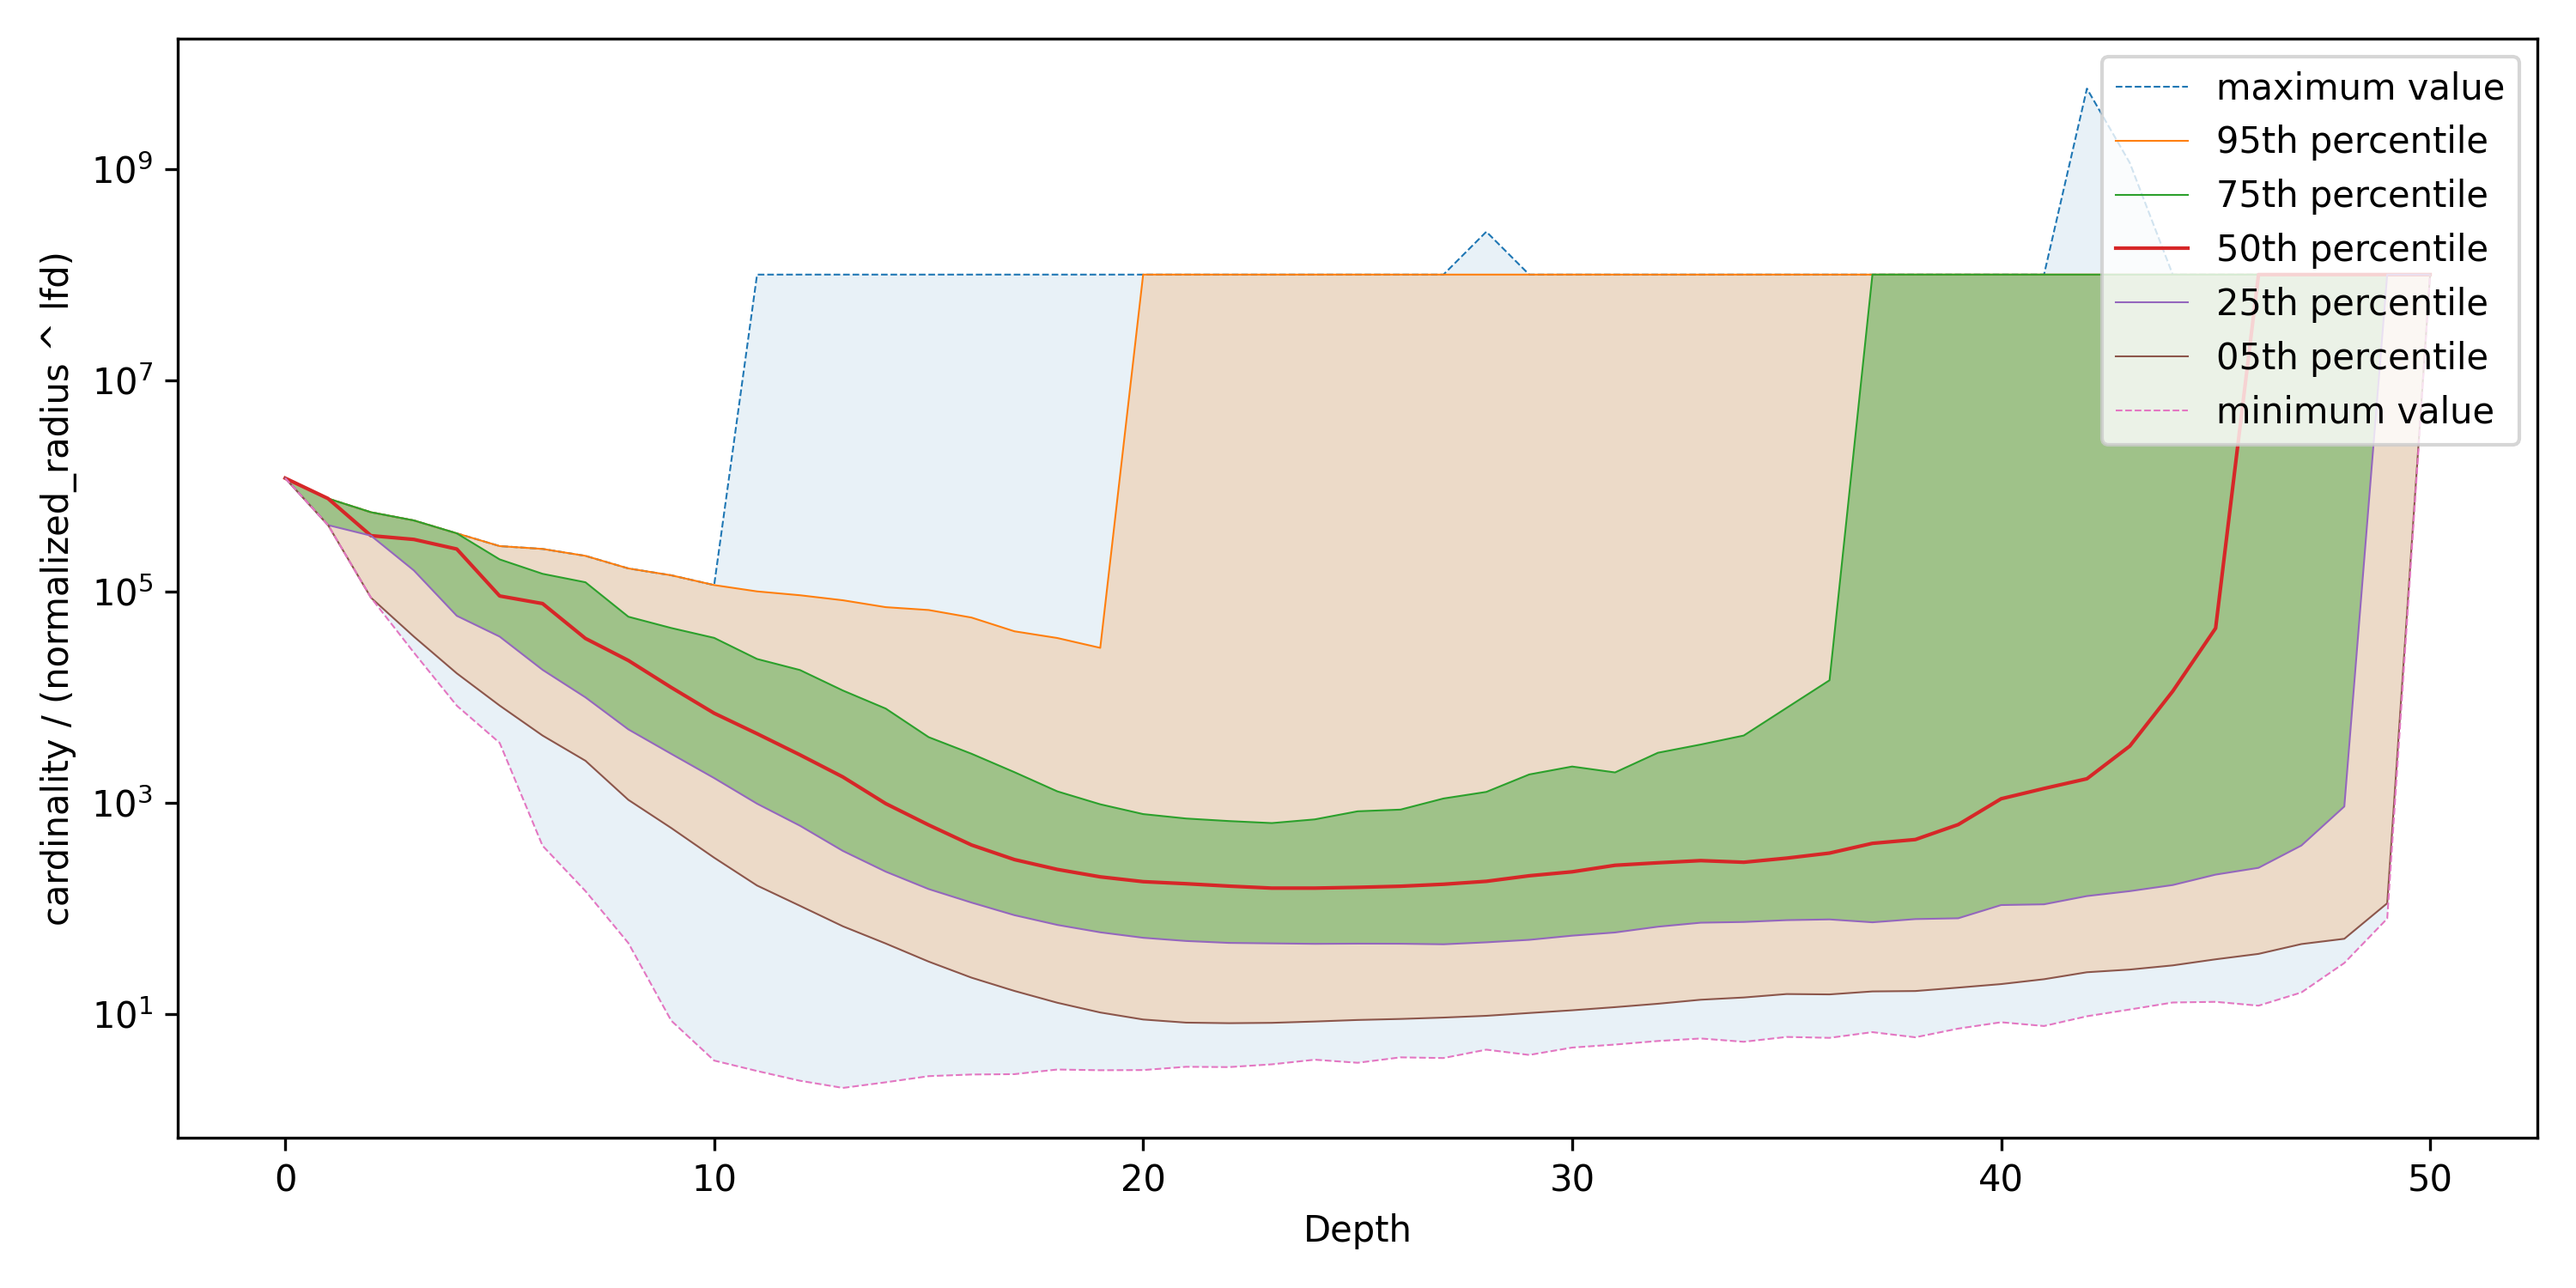
\includegraphics[width=0.95\textwidth]{images/fractal_density/glove-25-1183514.png}\\
    \subcaption{Glove-25}
    \label{fig:results:glove-25-fractal_density}
    \end{subfigure}
    \vspace{1em}
    \\
    \begin{subfigure}[b]{0.47\textwidth}
    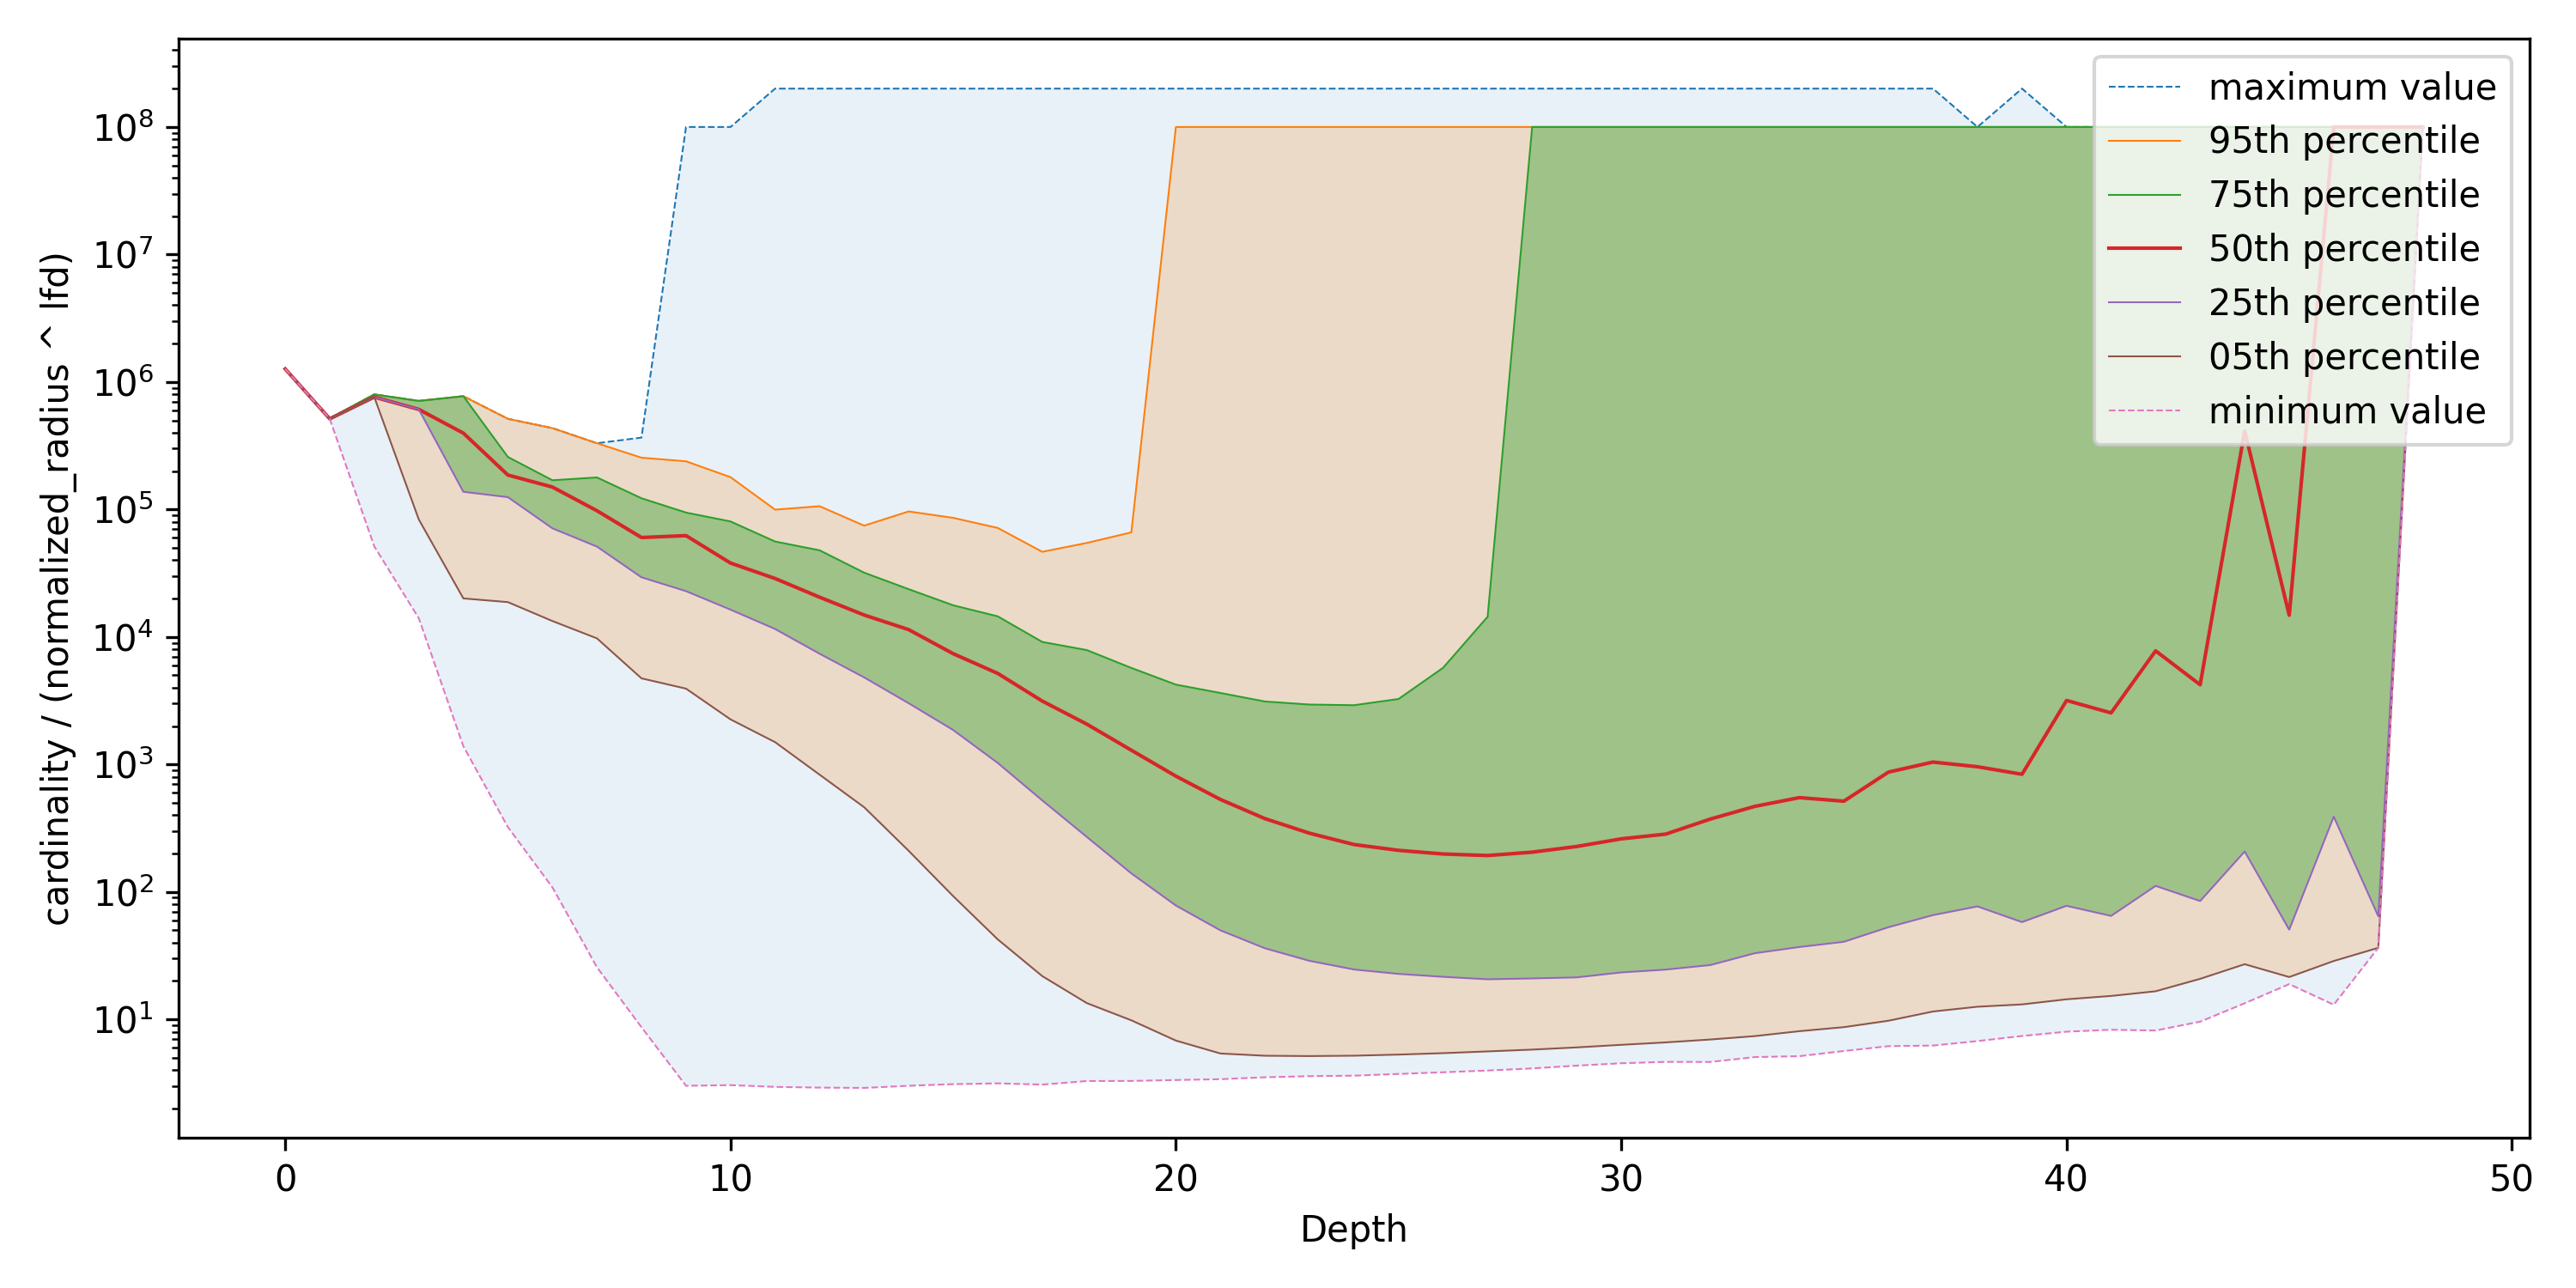
\includegraphics[width=0.95\textwidth]{images/fractal_density/sift-1000000.png}\\
    \subcaption{Sift}
    \label{fig:results:sift-fractal_density}
    \end{subfigure}%
    \begin{subfigure}[b]{0.47\textwidth}
    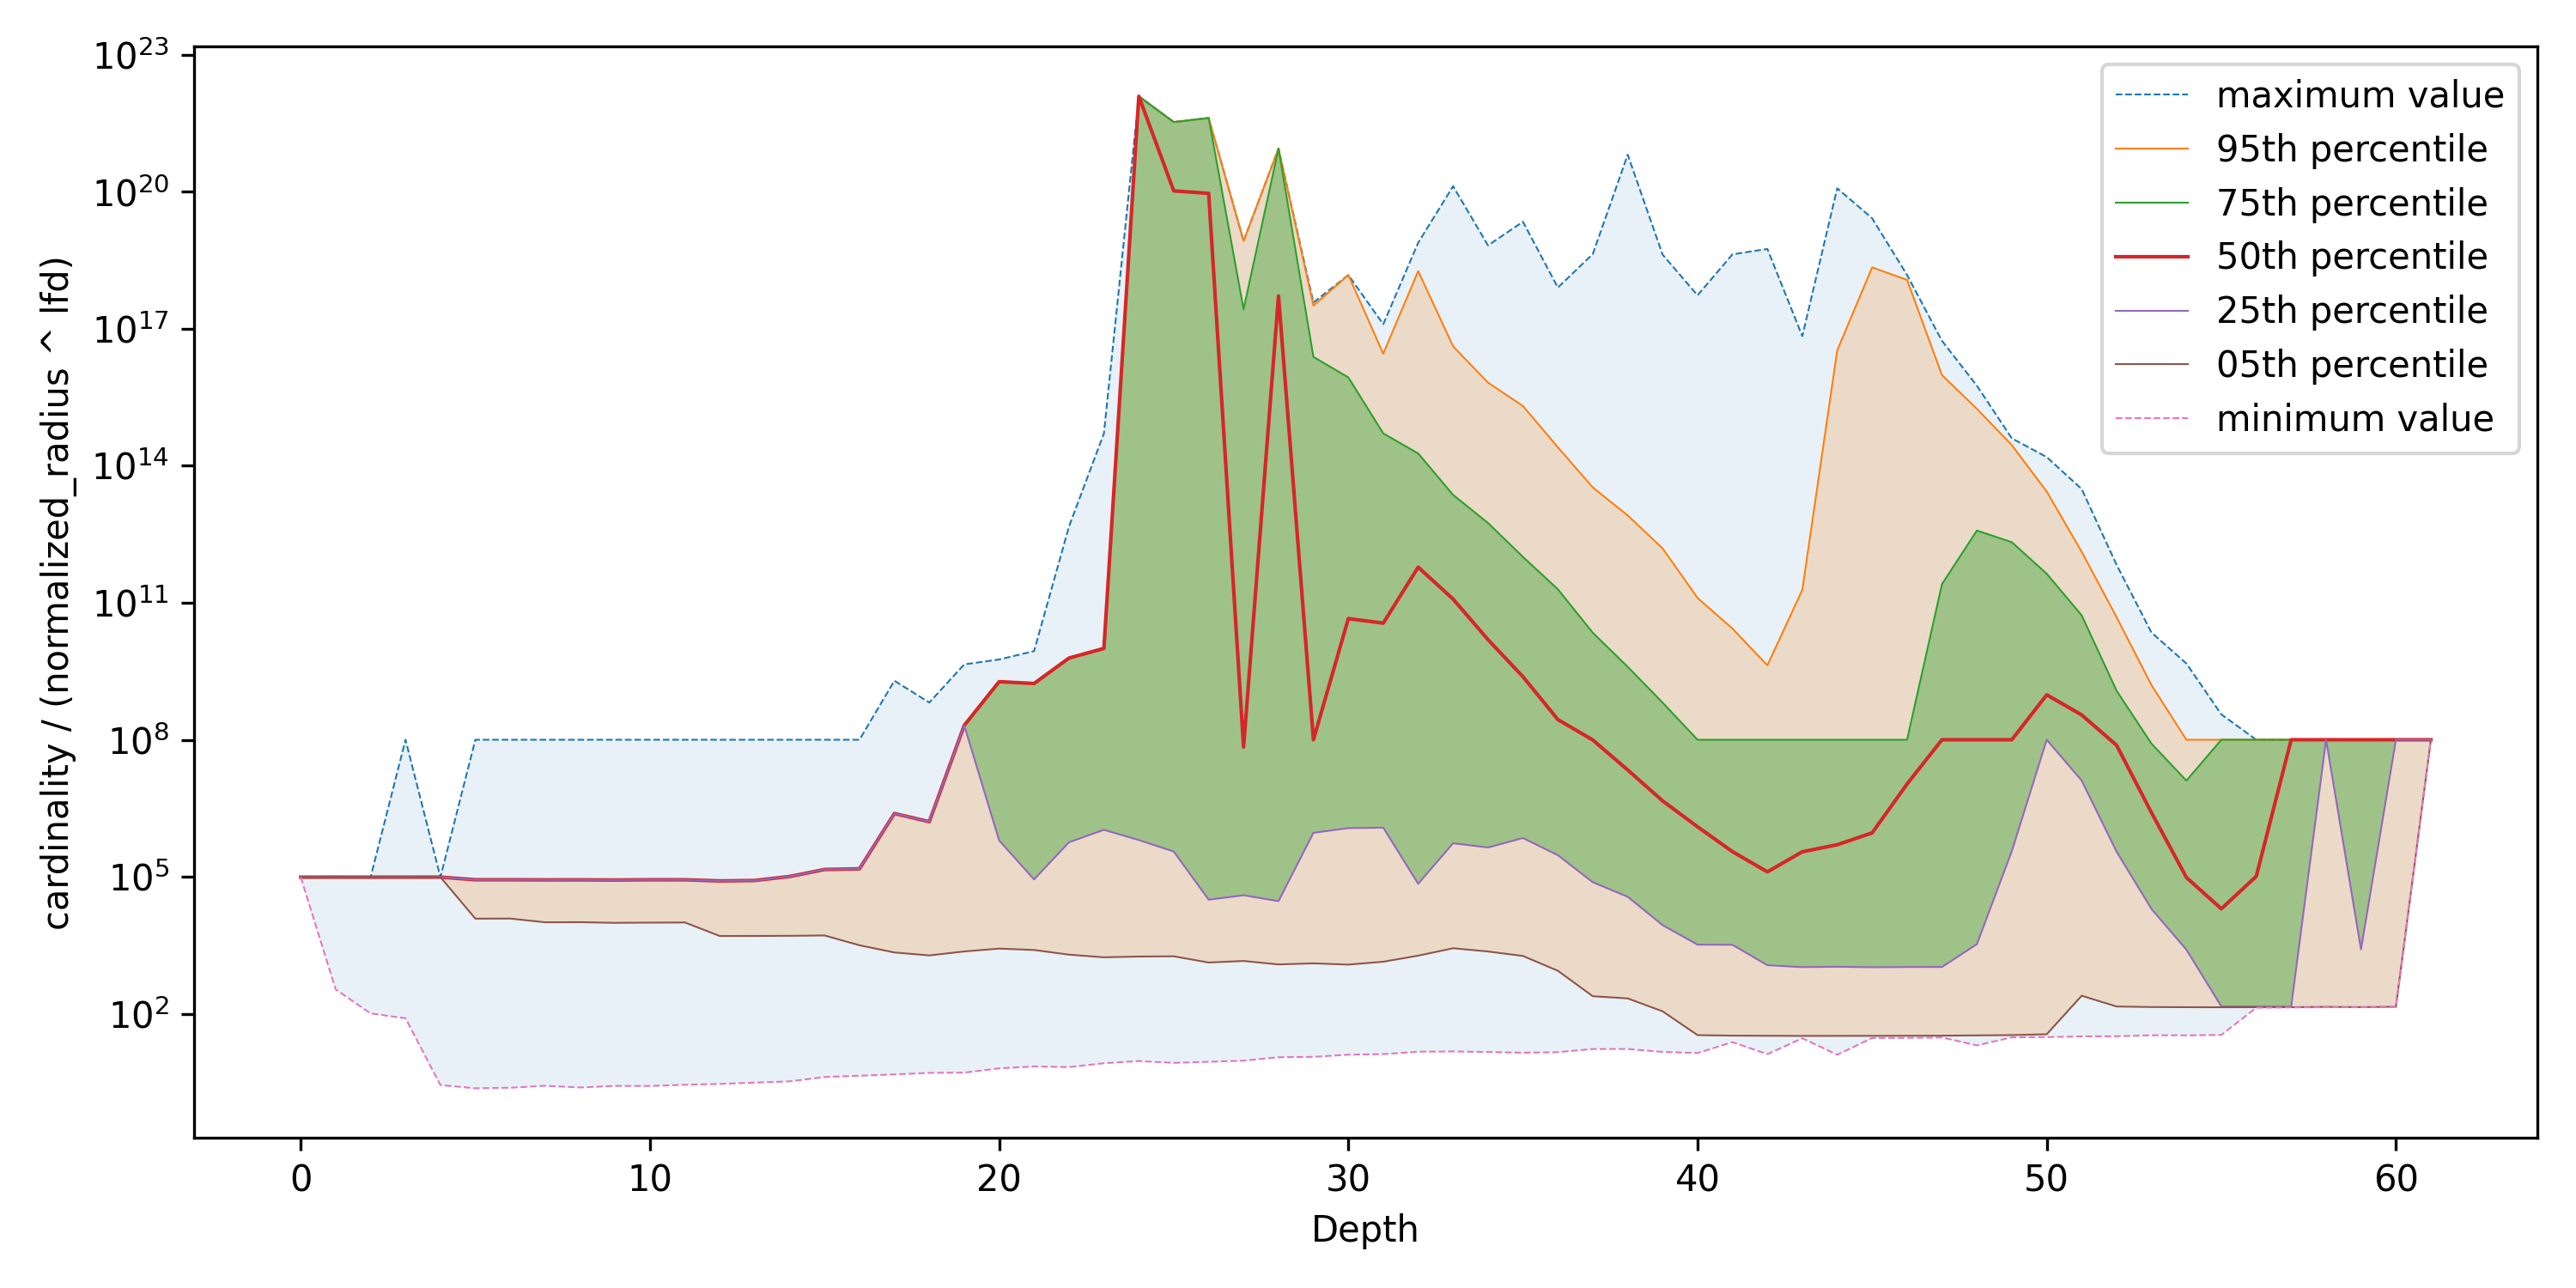
\includegraphics[width=0.95\textwidth]{images/fractal_density/radio-ml-97920.png}\\
    \subcaption{RadioML}
    \label{fig:results:radioml-fractal_density}
    \end{subfigure}%
    \\
    \begin{subfigure}[b]{0.47\textwidth}
    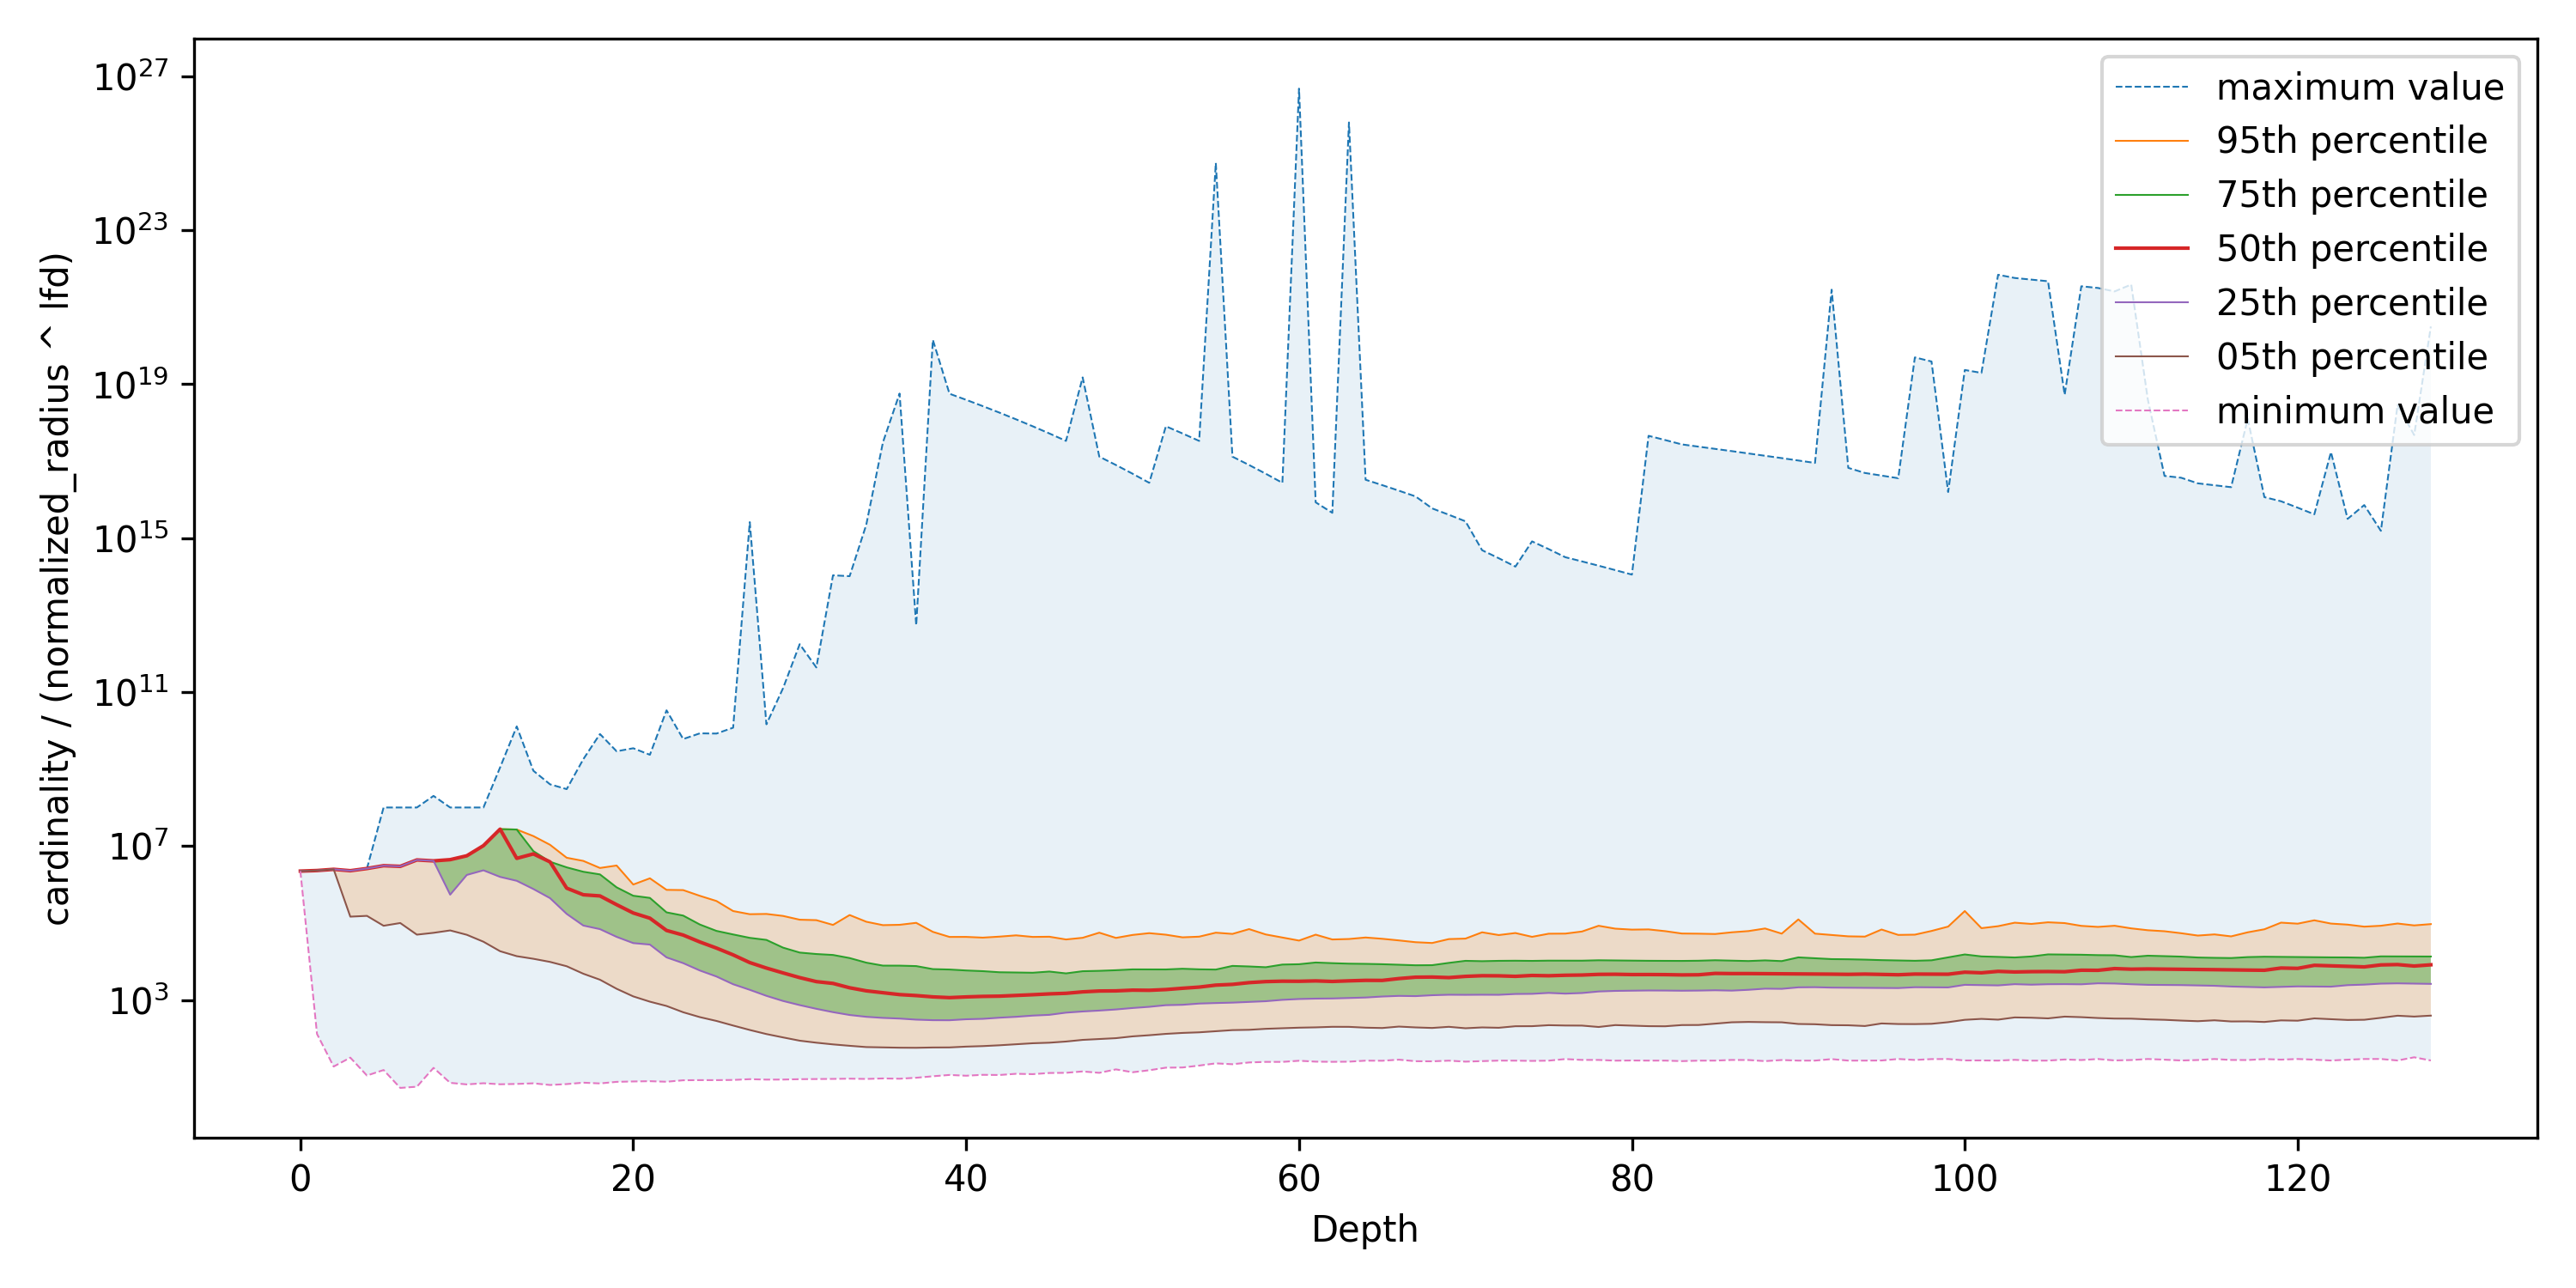
\includegraphics[width=0.95\textwidth]{images/fractal_density/silva-2224640.png}\\
    \subcaption{Silva 18S}
    \label{fig:results:silva-fractal_density}
    \end{subfigure}%  
    \begin{subfigure}[b]{0.47\textwidth}
    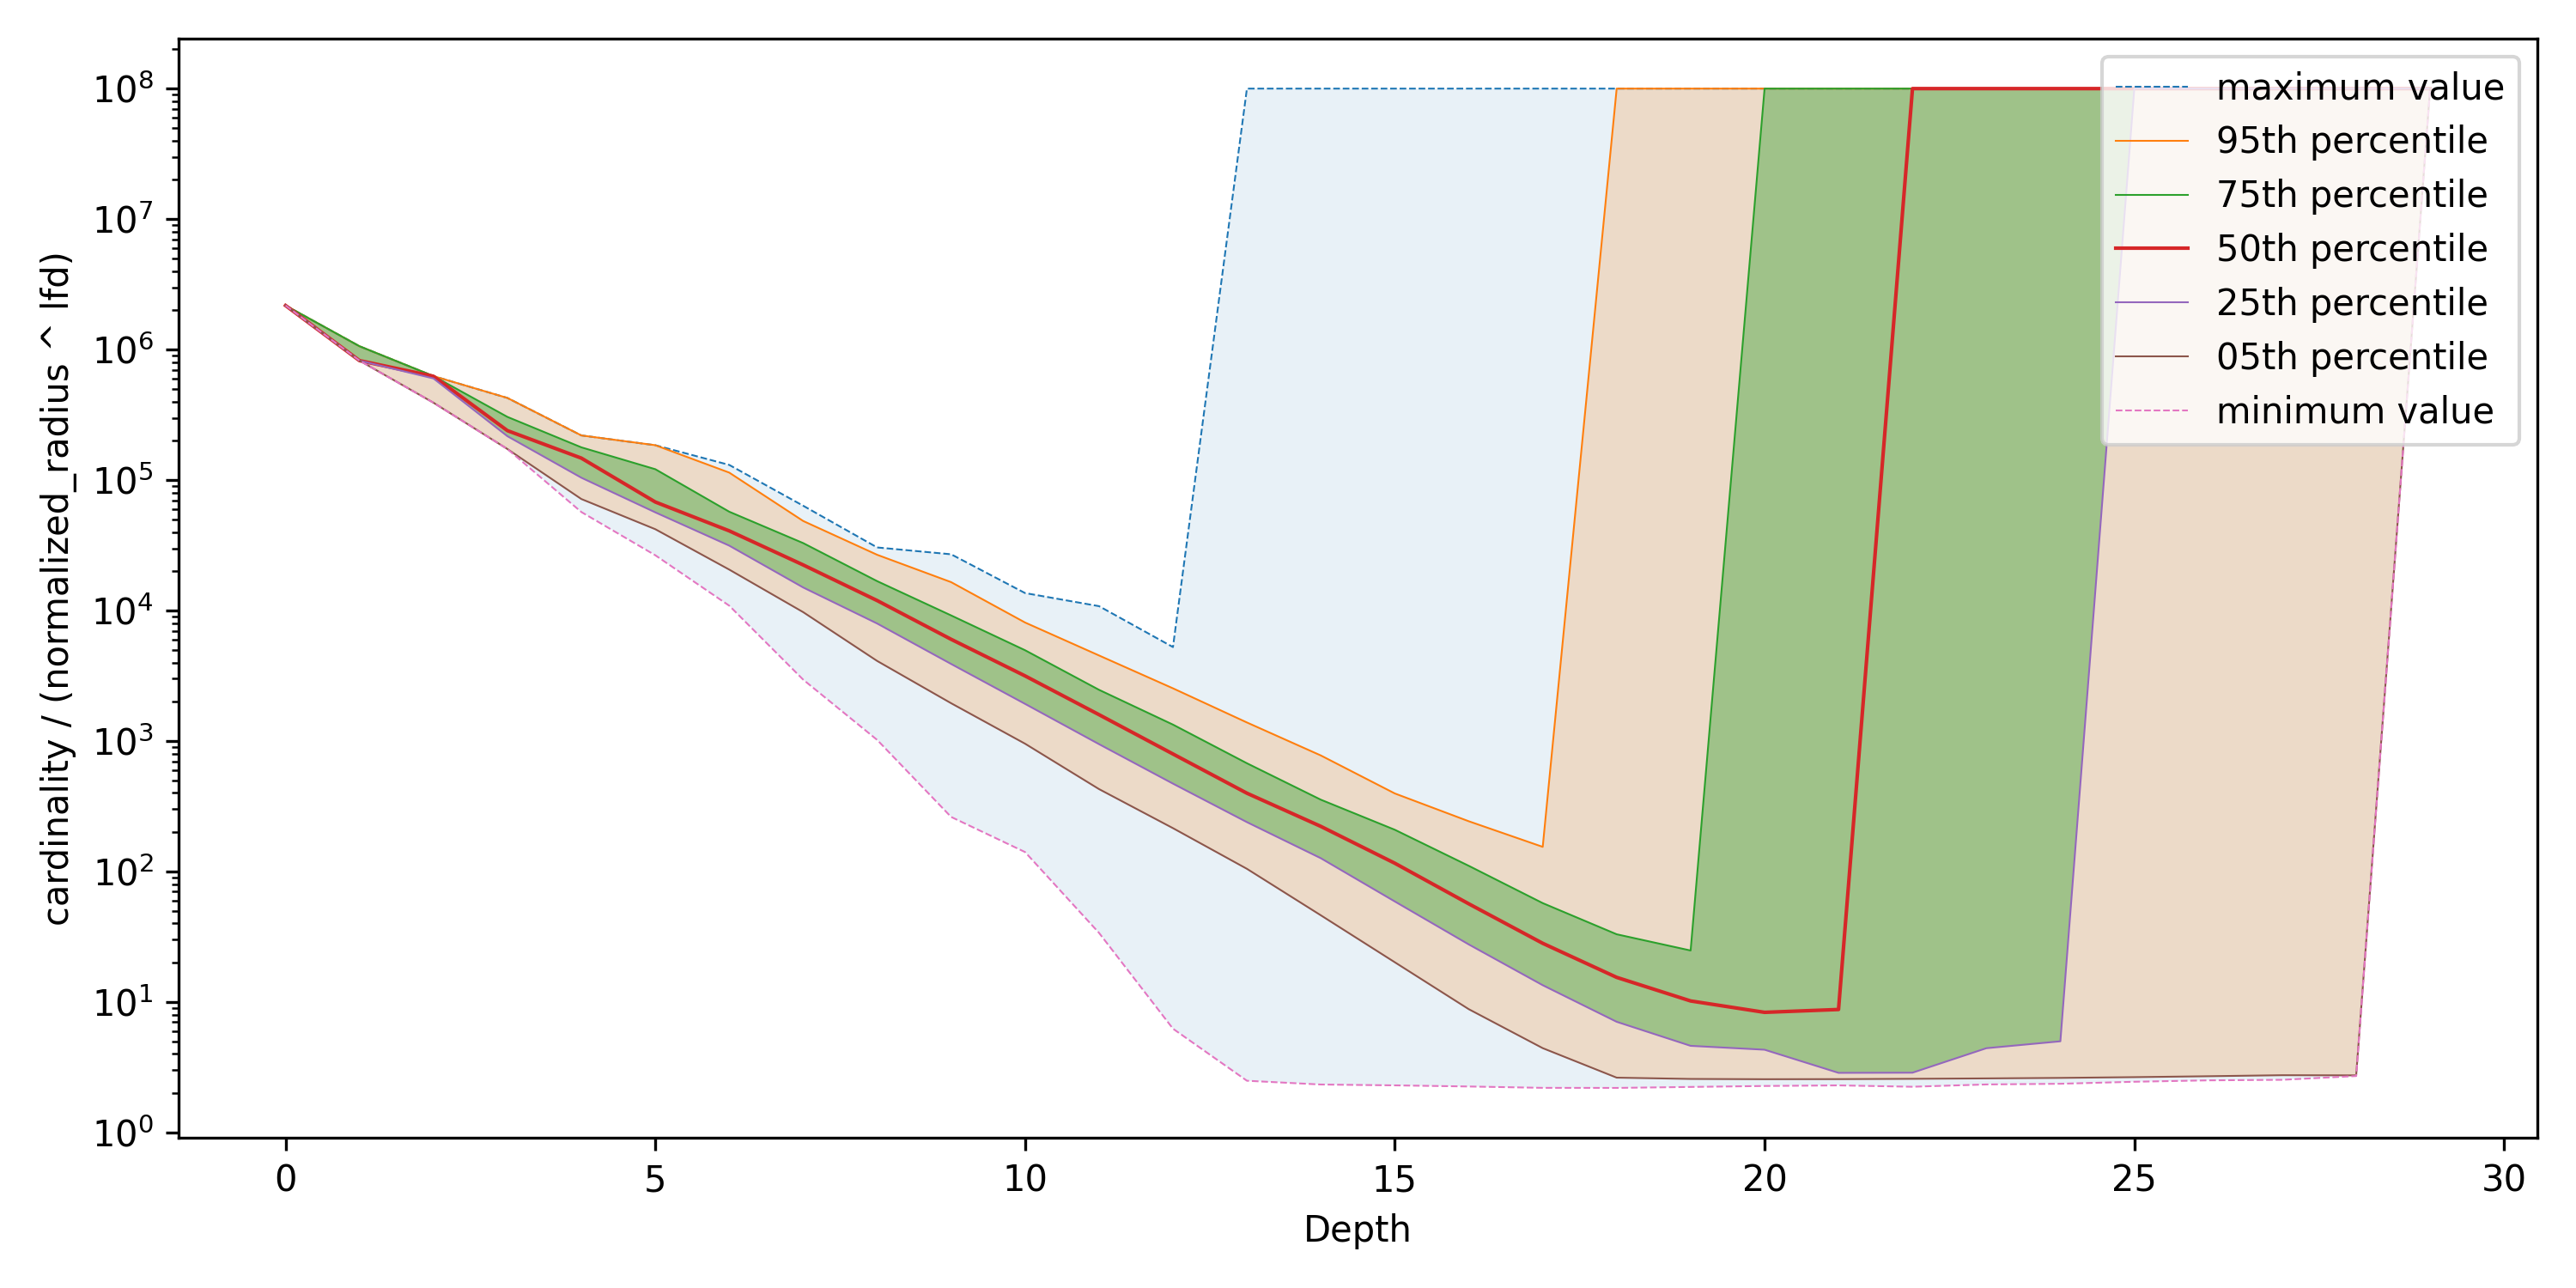
\includegraphics[width=0.95\textwidth]{images/fractal_density/random-1000000.png}\\
    \subcaption{A random dataset}
    \label{fig:results:random-fractal_density}
    \end{subfigure}
    \vspace{1em}
    \caption{Fractal Density vs. cluster depth across six datasets, grouped by decile of fractal density and weighted by the cardinalities of the clusters.
    The last dataset is randomly generated.
    Fractal Density is defined as $\frac{cardinality}{radius^{LFD}}$}
    \label{fig:results:fractal_density-plots}
\end{figure}
% 
% \end{document}